% AE 541 Assignment 1 - AIAA journal manuscript (submission version).
% Uses the official AIAA LaTeX template (new-aiaa.cls, new-aiaa.bst) in this folder.
% The "journal" option gives the required single-column, double-spaced, 10-pt layout.
\documentclass[journal]{new-aiaa}

\usepackage{graphicx}
\usepackage{amsmath}
\usepackage{booktabs}
\usepackage{multirow}
\usepackage{longtable,tabularx}
\usepackage{xcolor}
\usepackage{listings}
\setlength\LTleft{0pt}

% Shared macros for both report versions. Needs graphicx, listings, xcolor.
\RequirePackage{adjustbox}
\graphicspath{{../code/outputs/figures/}}

% public repository with the code, results and report sources
\newcommand{\repourl}{\url{https://github.com/BahaaIbrahimK/AE541-Assignment1-Surrogate-Modeling}}

% package versions printed by the script (outputs/summary.json)
\newcommand{\pyver}{3.11.9}
\newcommand{\npver}{2.4.6}
\newcommand{\spver}{1.17.1}
\newcommand{\skver}{1.9.1}
\newcommand{\mplver}{3.11.2}
\newcommand{\pdver}{3.0.6}

\definecolor{codebg}{RGB}{248,248,248}
\definecolor{codecomment}{RGB}{0,110,60}
\definecolor{codekeyword}{RGB}{20,60,160}
\definecolor{codestring}{RGB}{160,40,40}
\lstdefinestyle{pythoncode}{
  language=Python,
  basicstyle=\ttfamily\scriptsize,
  backgroundcolor=\color{codebg},
  commentstyle=\color{codecomment}\itshape,
  keywordstyle=\color{codekeyword}\bfseries,
  stringstyle=\color{codestring},
  numbers=left, numberstyle=\tiny\color{gray}, numbersep=6pt,
  frame=single, rulecolor=\color{black!25},
  breaklines=true, breakatwhitespace=false,
  postbreak=\mbox{\textcolor{gray}{$\hookrightarrow$}\space},
  showstringspaces=false, tabsize=4, columns=fullflexible, keepspaces=true,
  upquote=true,
  literate={φ}{{$\phi$}}1 {σ}{{$\sigma$}}1 {–}{{--}}1 {—}{{---}}1
}

\hypersetup{hidelinks}   % keep the links, drop the colored boxes around them

\title{Surrogate Modeling of the Rosenbrock and Trid Functions:\\Construction, Validation, and Limits of Trust}

\author{Bahaa Karawia\footnote{PhD Student, Aerospace Engineering Department; KFUPM ID 202510630. AE 541 Digital Twin in Modern Engineering, Assignment 1; assigned function (Part B): Trid function, 2 variables.}}
\affil{King Fahd University of Petroleum and Minerals, Dhahran 31261, Saudi Arabia}

\begin{document}

\maketitle

\begin{center}
  \small\singlespacing
  AE 541 Digital Twin in Modern Engineering \textbullet{} Assignment 1\\
  Bahaa Karawia, KFUPM ID 202510630 \textbullet{} Assigned function: Trid (2 variables)
\end{center}

\begin{abstract}
Two benchmark functions are treated as expensive simulations to test how far a cheap surrogate can be trusted. For the Rosenbrock function (common) and the two-variable Trid function (assigned), 60 evaluations from a maximin Latin hypercube design are split into 45 training and 15 held-out test points. Three surrogates are compared: polynomial regression with its degree chosen by five-fold cross-validation on the training set only, a cubic radial basis function (RBF) interpolant, and a Gaussian process (GP). They are assessed with test metrics, side-by-side error maps, learning curves, surrogate-based optimization with verification, and a reduced-box extrapolation test. Cross-validation recovers the true polynomial degrees (4 and 2), and the fitted coefficients match the exact expansions to within $4\times10^{-13}$. The GP reaches a test normalized root-mean-square error of $7.8\times10^{-6}$ and $1.0\times10^{-6}$ and places the two minima within 0.013 and $6\times10^{-4}$ of the truth. The RBF fails at the domain boundaries and creates a spurious negative minimum in the Rosenbrock valley, which only verification exposes. Outside a reduced training box, errors grow by factors of up to 2300. The hand-derived Trid minimum, $f=-2$ at $(2,2)$, is confirmed analytically and numerically.

\end{abstract}

\section*{Nomenclature}

{\renewcommand\arraystretch{1.0}
\noindent\begin{longtable*}{@{}l @{\quad=\quad} l@{}}
$\mathbf{A},\ \mathbf{P}$ & RBF kernel matrix and linear-tail matrix \\
$d$ & distance from a surrogate minimum to the known minimum \\
$f,\ \hat f$ & true function and surrogate prediction \\
$\mathcal{F}_k$ & $k$-th cross-validation fold \\
$\mathbf{H}$ & Hessian matrix \\
$k(\cdot,\cdot),\ \mathbf{K},\ \mathbf{k}_*$ & GP kernel, training covariance matrix, and training--test covariances \\
$\ell_j$ & GP length scale of input $j$ \\
$N,\ n,\ n_v$ & main DOE budget, number of training points, number of validation points \\
$n_{\mathrm{terms}}$ & number of polynomial coefficients \\
$p$ & total degree of the polynomial surrogate \\
$R^2$ & coefficient of determination \\
$\mu_j,\ s_j$ & training mean and standard deviation of input $j$ (scaling) \\
$\mathbf{u}$ & design point in unit-square coordinates \\
$\mathbf{x},\ \mathbf{z}$ & physical and standardized inputs \\
$\mathbf{x}^*$ & location of the global minimum \\
$\boldsymbol{\beta}$ & polynomial coefficients \\
$\varepsilon_{\mathrm{gen}}$ & generalization error \\
$\hat\mu,\ \hat\sigma$ & GP posterior mean and standard deviation \\
$\pi_j$ & random permutation used by the Latin hypercube \\
$\sigma_f^2,\ \sigma_n^2$ & GP signal and noise variances \\
$\phi_{\min}$ & minimum pairwise distance (maximin criterion) \\
$\boldsymbol{\psi},\ \boldsymbol{\Psi}$ & vector of monomials and polynomial design matrix \\
$w_i,\ c_j$ & RBF weights and linear-tail coefficients \\
CV & cross-validation \\
DOE & design of experiments \\
GP & Gaussian process \\
LHS & Latin hypercube sampling \\
MAE, MaxAE & mean and maximum absolute error \\
(N)RMSE & (normalized) root-mean-square error \\
RBF & radial basis function

\end{longtable*}}
% longtable* steps the table counter although it has no caption
\addtocounter{table}{-1}

% =====================================================================
% Shared body of the AE 541 Assignment 1 report (Bahaa Karawia, 202510630).
% Included by report_AIAA/202510630_Bahaa_Karawia.tex and by
% report_normal/202510630_Bahaa_Karawia_KFUPM.tex. Every number below is
% produced by code/202510630_Bahaa_Karawia.py (seed 7).
% =====================================================================

\section{Introduction}\label{sec:intro}

High-fidelity analyses such as CFD, finite-element models and coupled aero-structural solvers are too expensive to call thousands of times inside a design loop. The usual answer is a \emph{surrogate model}: a cheap approximation fitted to a small, deliberately chosen set of expensive runs, which then stands in for the analysis during exploration and optimization~\cite{queipo2005,forrester2008}. A surrogate is useful only if the engineer can say how wrong it is and where. The question behind this study is therefore not ``how low can the error go'' but ``can a cheap model guide a design decision reliably, and inside which bounds''~\cite{ae541brief}.

Two known two-variable functions are treated as if they were expensive simulations. Part~A uses the Rosenbrock function~\cite{rosenbrock1960}, common to the whole class; Part~B uses the two-variable Trid function~\cite{sfu_vlse}, assigned to the author. Because both functions are known everywhere, every claim a surrogate makes can be checked against the truth, a luxury that a real project never has. For each function the complete workflow of the course reference notebook~\cite{ae541tutorial} is applied: definition of the function and domain, design of experiments (DOE), a leakage-free train/test split, three surrogate types, complexity selection by training-only cross-validation (CV), held-out validation, side-by-side error maps, uncertainty quantification, learning curves, surrogate-based optimization with verification, and an extrapolation test. The shared theory is given once in Sec.~\ref{sec:method}; results for the two functions follow in Secs.~\ref{sec:rosen} and~\ref{sec:trid}, and Sec.~\ref{sec:discussion} compares them and states where each model can be trusted.

% ---------------------------------------------------------------------
\section{Methodology}\label{sec:method}

\subsection{Problem Statement}

Let the expensive model be a deterministic map $f:\mathcal{X}\subset\mathbb{R}^2\rightarrow\mathbb{R}$ on the box $\mathcal{X}=[l_1,u_1]\times[l_2,u_2]$. From a design $\mathcal{D}=\{(\mathbf{x}^{(i)},y^{(i)})\}_{i=1}^{N}$ with $y^{(i)}=f(\mathbf{x}^{(i)})$, a surrogate $\hat f(\mathbf{x};\boldsymbol{\theta})\approx f(\mathbf{x})$ is built. The quantity of interest is the generalization error over the whole domain,
\begin{equation}
  \varepsilon_{\mathrm{gen}}^2=\frac{1}{|\mathcal{X}|}\int_{\mathcal{X}}\big(f(\mathbf{x})-\hat f(\mathbf{x})\big)^2\,\mathrm{d}\mathbf{x}.
  \label{eq:gen}
\end{equation}
Equation~\eqref{eq:gen} needs $f$ everywhere, so in practice it can only be \emph{estimated} from data the model has not seen (a held-out test set, or CV). Here it can also be evaluated on a dense $120\times120$ grid, which is used purely as a diagnostic.

The two functions are listed in Table~\ref{tab:functions}. Both are polynomials: expanding the squares gives
\begin{align}
  f_{\mathrm{R}}(x_1,x_2) &= 100(x_2-x_1^2)^2+(1-x_1)^2 = 100x_1^4-200x_1^2x_2+100x_2^2+x_1^2-2x_1+1, \label{eq:rosen}\\
  f_{\mathrm{T}}(x_1,x_2) &= (x_1-1)^2+(x_2-1)^2-x_1x_2 = x_1^2+x_2^2-x_1x_2-2x_1-2x_2+2, \label{eq:trid}
\end{align}
so the Rosenbrock function is exactly of total degree 4 and the Trid function exactly of degree 2. This fact is known here but is \emph{not} used to choose any model setting; Sec.~\ref{sec:tuning} shows that CV recovers it from the data alone.

\begin{table}[!htbp]
  \centering
  \caption{Test functions, domains, known global minima and the exact range of $f$ on each box.}
  \label{tab:functions}
  \begin{adjustbox}{max width=\linewidth}
  \begin{tabular}{lccccc}
    \toprule
    Function & Domain & $\mathbf{x}^*$ & $f(\mathbf{x}^*)$ & Range of $f$ & Exact degree \\
    \midrule
    Rosenbrock, Eq.~\eqref{eq:rosen} & $[-2,2]^2$ & $(1,\,1)$ & $0$ & $0$ to $3609$ & 4 \\
    Trid, Eq.~\eqref{eq:trid} & $[-4,4]^2$ & $(2,\,2)$ & $-2$ & $-2$ to $50$ & 2 \\
    \bottomrule
  \end{tabular}
  \end{adjustbox}
\end{table}

\subsection{Design of Experiments}\label{sec:doe_method}

The main budget is $N=60$ evaluations, counting training and test points together. All designs are generated in the unit square and mapped linearly to the physical box, so their space-filling quality can be compared independently of the domain size. Three designs are compared at the same $N$: uniform random sampling; a Latin hypercube (LHS), which splits each axis into $N$ bins and places exactly one point in each bin~\cite{mckay1979},
\begin{equation}
  u^{(i)}_j=\frac{\pi_j(i)-1+U_{ij}}{N},\qquad U_{ij}\sim\mathcal{U}(0,1),
  \label{eq:lhs}
\end{equation}
where $\pi_j$ is a random permutation of $\{1,\dots,N\}$; and a \emph{maximin LHS}, the best of 100 independent LHS draws under the maximin criterion~\cite{johnson1990}
\begin{equation}
  \phi_{\min}=\min_{i\neq k}\big\|\mathbf{u}^{(i)}-\mathbf{u}^{(k)}\big\|_2 .
  \label{eq:maximin}
\end{equation}
Generating candidate designs costs no function evaluations, so screening them improves the spread for free while keeping the one-dimensional stratification of the LHS. Equations~\eqref{eq:lhs} and~\eqref{eq:maximin} are written in unit-square coordinates, so $\phi_{\min}$ can be compared between the two boxes. To avoid judging the designs on a single lucky draw, $\phi_{\min}$ is also computed for 500 independent random and LHS realizations.

\subsection{Train/Test Split and Data Leakage}\label{sec:split}

The 60 samples are split once, at random (seed 7), into 45 training and 15 test points. The test points are set aside immediately and are used only after every modeling choice has been fixed. \emph{Data leakage} means that information from the test data reaches the fitting process, for example when the input scaling ($\mu_j,s_j$) is computed from all 60 points, or when a degree or kernel bound is chosen by looking at test error; either makes the reported error optimistic. It is avoided here in three ways: (i) the standardization $z_j=(x_j-\mu_j)/s_j$ sits inside a scikit-learn pipeline~\cite{pedregosa2011}, so every fit, including each CV fold, learns $\mu_j$ and $s_j$ from its own training rows only; (ii) the polynomial degree and the GP bound study (Sec.~\ref{sec:gp_method}) are judged by training-only CV; (iii) test and dense-grid errors are reported as diagnostics and never fed back.

\subsection{Surrogate Models}\label{sec:models}

\paragraph{Polynomial regression (required).} A total-degree-$p$ polynomial in the standardized inputs,
\begin{equation}
  \hat f(\mathbf{x})=\sum_{a+b\le p}\beta_{ab}\,z_1^a z_2^b=\boldsymbol{\psi}(\mathbf{z})^{\mathsf T}\boldsymbol{\beta},
  \qquad n_{\mathrm{terms}}=\frac{(p+1)(p+2)}{2},
  \label{eq:poly}
\end{equation}
is fitted by least squares, $\boldsymbol{\beta}^*=\arg\min\|\mathbf{y}-\boldsymbol{\Psi}\boldsymbol{\beta}\|_2^2$, where the rows of the design matrix $\boldsymbol{\Psi}$ are the monomials $\boldsymbol{\psi}(\mathbf{z}^{(i)})^{\mathsf T}$. The coefficients $\beta_{ab}$ are the only parameters. The system is solved by an SVD-based least-squares routine; when $n_{\mathrm{terms}}$ exceeds the number of points, the problem is under-determined and this routine returns the minimum-norm solution, one of infinitely many exact fits. Because an affine input scaling preserves the degree, the fitted model is also an exact degree-$p$ polynomial in the physical $\mathbf{x}$; its physical coefficients are recovered by projecting $\hat f$ onto the raw monomials on the grid, which allows a direct comparison with Eqs.~\eqref{eq:rosen} and~\eqref{eq:trid}.

\paragraph{Cubic radial basis function (RBF) interpolation.} The RBF model is a weighted sum of radially symmetric kernels centered on the $n$ training points, plus a linear tail~\cite{buhmann2003}:
\begin{equation}
  \hat f(\mathbf{z})=\sum_{i=1}^{n}w_i\,\big\|\mathbf{z}-\mathbf{z}^{(i)}\big\|^3+c_0+c_1z_1+c_2z_2,
  \qquad \sum_i w_i=0,\quad \sum_i w_i\,\mathbf{z}^{(i)}=\mathbf{0}.
  \label{eq:rbf}
\end{equation}
The side conditions in Eq.~\eqref{eq:rbf} stop the weights from carrying a linear trend of their own. Imposing $\hat f(\mathbf{z}^{(i)})=y^{(i)}$ gives the symmetric saddle-point system
\begin{equation}
  \begin{bmatrix}\mathbf{A}&\mathbf{P}\\\mathbf{P}^{\mathsf T}&\mathbf{0}\end{bmatrix}
  \begin{bmatrix}\mathbf{w}\\\mathbf{c}\end{bmatrix}=
  \begin{bmatrix}\mathbf{y}\\\mathbf{0}\end{bmatrix},
  \qquad A_{ik}=\big\|\mathbf{z}^{(i)}-\mathbf{z}^{(k)}\big\|^3,\quad \mathbf{P}=[\mathbf{1},\,\mathbf{z}_1,\,\mathbf{z}_2].
  \label{eq:rbf_sys}
\end{equation}
The weights $w_i$ and tail coefficients $c_0,c_1,c_2$, obtained by solving Eq.~\eqref{eq:rbf_sys}, are the parameters; the cubic kernel has no shape parameter to tune. The model interpolates the data exactly, which is appropriate for deterministic simulations, but it reproduces exactly only polynomials of degree at most one (the tail).

\paragraph{Gaussian process (GP) regression.}\label{sec:gp_method} The outputs are modeled as a GP with a squared-exponential kernel with automatic relevance determination (ARD) and a small noise term~\cite{rasmussen2006}:
\begin{equation}
  k(\mathbf{z},\mathbf{z}')=\sigma_f^2\exp\!\left(-\frac12\sum_{j=1}^{2}\frac{(z_j-z'_j)^2}{\ell_j^2}\right)+\sigma_n^2\,\delta_{\mathbf{z}\mathbf{z}'} .
  \label{eq:kernel}
\end{equation}
In Eq.~\eqref{eq:kernel}, $\sigma_f^2$ is the signal variance (how far the normalized output swings), $\ell_j$ is the length scale of input $j$ (how far one must move in $z_j$ before the output changes appreciably, so a small $\ell_j$ marks a sensitive direction), and $\sigma_n^2$ absorbs numerical noise. With $\mathbf{K}=k(\mathbf{Z},\mathbf{Z})$ and $\mathbf{k}_*=k(\mathbf{Z},\mathbf{z}_*)$, the posterior mean and variance are
\begin{equation}
  \hat\mu(\mathbf{z}_*)=\mathbf{k}_*^{\mathsf T}\mathbf{K}^{-1}\mathbf{y},\qquad
  \hat\sigma^2(\mathbf{z}_*)=k(\mathbf{z}_*,\mathbf{z}_*)-\mathbf{k}_*^{\mathsf T}\mathbf{K}^{-1}\mathbf{k}_* .
  \label{eq:gp}
\end{equation}
The hyperparameters $\boldsymbol{\theta}=(\sigma_f,\ell_1,\ell_2,\sigma_n)$ maximize the log marginal likelihood
\begin{equation}
  \log p(\mathbf{y}\mid\mathbf{Z},\boldsymbol{\theta})=-\tfrac12\mathbf{y}^{\mathsf T}\mathbf{K}^{-1}\mathbf{y}-\tfrac12\log|\mathbf{K}|-\tfrac{n}{2}\log2\pi .
  \label{eq:lml}
\end{equation}
Equation~\eqref{eq:lml} is maximized with normalized outputs, eight random restarts (nine optimizer runs in total), and the bounds $\sigma_f^2\in[10^{-3},10^4]$, $\ell_j\in[10^{-2},10^3]$ and $\sigma_n^2\in[10^{-12},10^{-2}]$; the initial values and all other settings are listed in the configuration block of the script. The GP was added as a third model because it provides the uncertainty estimate $\hat\sigma$ needed for step~9 of the assignment, and because it is the standard surrogate in aerospace design optimization~\cite{forrester2008,jones1998}. Whenever a hyperparameter ends at a bound, the fit is repeated with $\sigma_f^2\le10^6$ and $\le10^8$ and the alternatives are compared by training CV only. Optimizer runs that end with an abnormal line-search termination are counted and reported.

\subsection{Complexity Selection}\label{sec:tuning_method}

The polynomial degree $p$ of Eq.~\eqref{eq:poly} is swept over $p=1,\dots,8$ and scored by the pooled five-fold CV RMSE on the 45 training points,
\begin{equation}
  \mathrm{RMSE}_{\mathrm{CV}}=\sqrt{\frac{1}{n}\sum_{k=1}^{5}\sum_{i\in\mathcal{F}_k}\big(y^{(i)}-\hat f^{(-k)}(\mathbf{x}^{(i)})\big)^2},
  \label{eq:cv}
\end{equation}
where $\hat f^{(-k)}$ is refitted, scaler included, without fold $\mathcal{F}_k$~\cite{hastie2009}. The choice of $p$ is a bias--variance trade-off~\cite{hastie2009}: too low a degree leaves a systematic (bias) error that more data cannot remove, whereas too high a degree makes the fit sensitive to the particular sample (variance) and, numerically, to the conditioning of $\boldsymbol{\Psi}$. Each CV training fold holds 36 points, so degree 7 ($n_{\mathrm{terms}}=36$) is exactly determined and degree 8 ($n_{\mathrm{terms}}=45$) is under-determined inside the folds. With noiseless polynomial data every degree at or above the true one gives an error at round-off level, and the arg-min among those values is decided by floating-point noise. The selection rule is therefore a parsimony rule: choose the smallest $p$ whose CV RMSE is within 5\% of the best value, or below $10^{-9}\,\mathrm{std}(y_{\mathrm{train}})$, which is treated as exact. Only the CV error of Eq.~\eqref{eq:cv} enters the choice; the test and dense-grid errors are computed after the degree has been locked and are plotted only as diagnostics.

\subsection{Validation Metrics}

For $n_v$ validation points with truth $y_i$ and prediction $\hat y_i$,
\begin{equation}
  \mathrm{RMSE}=\sqrt{\tfrac{1}{n_v}\textstyle\sum_i(y_i-\hat y_i)^2},\quad
  \mathrm{MAE}=\tfrac{1}{n_v}\textstyle\sum_i|y_i-\hat y_i|,\quad
  R^2=1-\dfrac{\sum_i(y_i-\hat y_i)^2}{\sum_i(y_i-\bar y)^2},
  \label{eq:metrics1}
\end{equation}
\begin{equation}
  \mathrm{MaxAE}=\max_i|y_i-\hat y_i|,\qquad
  \mathrm{NRMSE}=\frac{\mathrm{RMSE}}{\max(y_{\mathrm{test}})-\min(y_{\mathrm{test}})} .
  \label{eq:metrics2}
\end{equation}
The metrics of Eqs.~\eqref{eq:metrics1} and~\eqref{eq:metrics2} are computed on the test set; on the dense grid, NRMSE is normalized by the range of the grid values instead. Every model is compared with the trivial baseline $\hat y=\mathrm{mean}(y_{\mathrm{train}})$; a surrogate that does not beat it has learned nothing. RMSE and MAE carry the units of $f$, NRMSE makes the two functions comparable, and MaxAE is the worst-case number that usually matters in design. CV is used to select, the test set gives the final independent check, and the dense grid shows what both estimates miss.

\subsection{Uncertainty, Sample Size, Optimization and Extrapolation}\label{sec:protocols}

\emph{Uncertainty.} The GP standard deviation $\hat\sigma$ of Eq.~\eqref{eq:gp} is mapped over the grid and compared with the true $|f-\hat f|$ through the Pearson and Spearman correlations and the fraction of grid points with $|f-\hat f|\le2\hat\sigma$. The small diagonal jitter $\alpha=10^{-10}$ that scikit-learn adds to $\mathbf{K}$ for numerical stability, together with $\sigma_n^2$, puts a floor of about $\sqrt{\alpha+\sigma_n^2}\,\mathrm{std}(y_{\mathrm{train}})$ under $\hat\sigma$; this floor is reported with the results.

\emph{Learning curve.} Each model is refitted on fresh LHS designs of $N=20,30,45,65,90$ training points, five independent draws per size, and scored by RMSE on the full grid and on a central box whose sides are 75\% of the domain sides (56\% of its area). The core score separates edge effects from interior accuracy. The polynomial keeps its CV-selected degree at every $N$ because $n_{\mathrm{terms}}\le20$ in both cases; no degree reduction was needed.

\emph{Optimization.} Each surrogate is minimized by bounded Nelder--Mead~\cite{nelder1965} from 20 LHS start points. Nelder--Mead is derivative free, which avoids the finite-difference failure on GP predictions noted in the reference notebook~\cite{ae541tutorial}. End points closer than 2\% of the box width (0.08 for Rosenbrock, 0.16 for Trid) are merged into one candidate. Each distinct candidate is then evaluated once with the true function, and the predicted value, the true value and the distance to the known minimum are tabulated. The known minimum is never inserted as a result. The same multi-start search on the true function confirms the reference minimum numerically.

\emph{Extrapolation.} Each model is retrained on 45 LHS points inside a reduced box (the central quarter of the domain by area) and evaluated over the full grid; errors inside and outside the training box are reported separately.

\subsection{Reproducibility}

All results come from the single script \texttt{202510630\_Bahaa\_Karawia.py} (Appendix~\ref{app:code}), run with Python~\pyver, NumPy~\npver~\cite{harris2020}, SciPy~\spver~\cite{virtanen2020}, scikit-learn~\skver~\cite{pedregosa2011}, Matplotlib~\mplver~\cite{hunter2007} and pandas~\pdver~\cite{mckinney2010}. The master seed is 7, and every random draw derives from it through fixed offsets set in the configuration block. The command \texttt{python 202510630\_Bahaa\_Karawia.py} writes every figure and table of this report to \texttt{./outputs} in about two minutes. The same unit-square design is used for both functions, so differences between Parts~A and~B come from the functions, not from the sampling.

The script, every generated figure and table, both versions of this report and the list of pinned package versions are available in the public repository
\begin{center}\repourl\end{center}
\noindent One command rebuilds everything from scratch: \texttt{reproduce.ps1} on Windows or \texttt{reproduce.sh} on Linux and macOS. On every change to the repository, an automated GitHub Actions job reruns the study on a clean Linux machine and checks the fresh results against the committed ones. The workflow and parts of the code (LHS, RBF system, GP set-up) are adapted from the course notebook~\cite{ae541tutorial}.

% ---------------------------------------------------------------------
\section{Results, Part A: Rosenbrock Function}\label{sec:rosen}

\subsection{Function, Domain and Minimum}

Figure~\ref{fig:R_truth} shows the Rosenbrock function on $[-2,2]^2$. The minimum $f=0$ at $(1,1)$ lies at the end of the curved ``banana'' valley $x_2=x_1^2$; the script checks $f(1,1)=0$ before any fitting. Across the valley the function rises steeply, reaching 3609 at the corner $(-2,-2)$, while along its floor it reduces to $(1-x_1)^2$ and varies only between 0 and 5.8. The interesting region (small $f$) is a thin curved band that covers a tiny fraction of the domain, so any global error metric will be dominated by the large corner values.

\begin{figure}[!htbp]
  \centering
  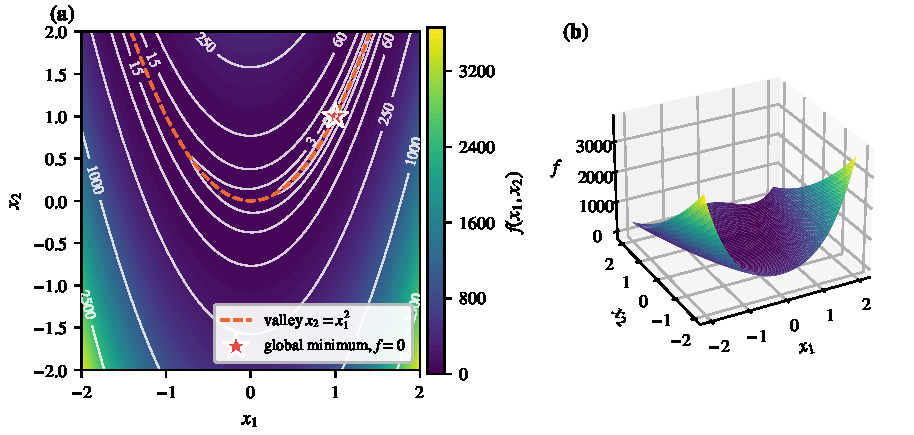
\includegraphics[width=\textwidth]{rosenbrock/fig01_truth.pdf}
  \caption{Rosenbrock function on $[-2,2]^2$. (a) Filled contour map with iso-lines at $f=0.5,3,15,60,250,1000,2500$; the dashed line is the valley floor $x_2=x_1^2$ and the star marks the global minimum $f=0$ at $(1,1)$. (b) Three-dimensional surface of the same field, with the minimum marked.}
  \label{fig:R_truth}
\end{figure}

\subsection{Design of Experiments}

The three designs of Sec.~\ref{sec:doe_method} are shown in Fig.~\ref{fig:doe}, and their maximin distances are listed in Table~\ref{tab:doe}. The single random design leaves visible holes and clusters and its axis projections (red ticks) pile up; the LHS projections are evenly spaced by construction. Over 500 realizations, the median $\phi_{\min}$ of LHS (0.0217) is almost twice that of random sampling (0.0115), and the 5th percentile is three times larger (0.0105 against 0.0035), so the LHS rarely produces the near-duplicate points that waste a random design. The maximin LHS used here reaches $\phi_{\min}=0.0452$, higher than every one of the 500 plain LHS draws (maximum 0.0432) and almost twice the random design at the same cost.

The budget $N=60$ was chosen from the models to be fitted. With 45 training points a degree-4 polynomial (15 coefficients) has three points per coefficient on the full training set and 2.4 per coefficient inside a CV fold, above the usual rule of thumb $n\ge2n_{\mathrm{terms}}$; the learning curve of Sec.~\ref{sec:R_learning} then confirms that the GP error falls by two orders of magnitude up to $N=45$ and only by a factor of three between 45 and 90, so a larger budget would buy comparatively little.

\begin{figure}[!htbp]
  \centering
  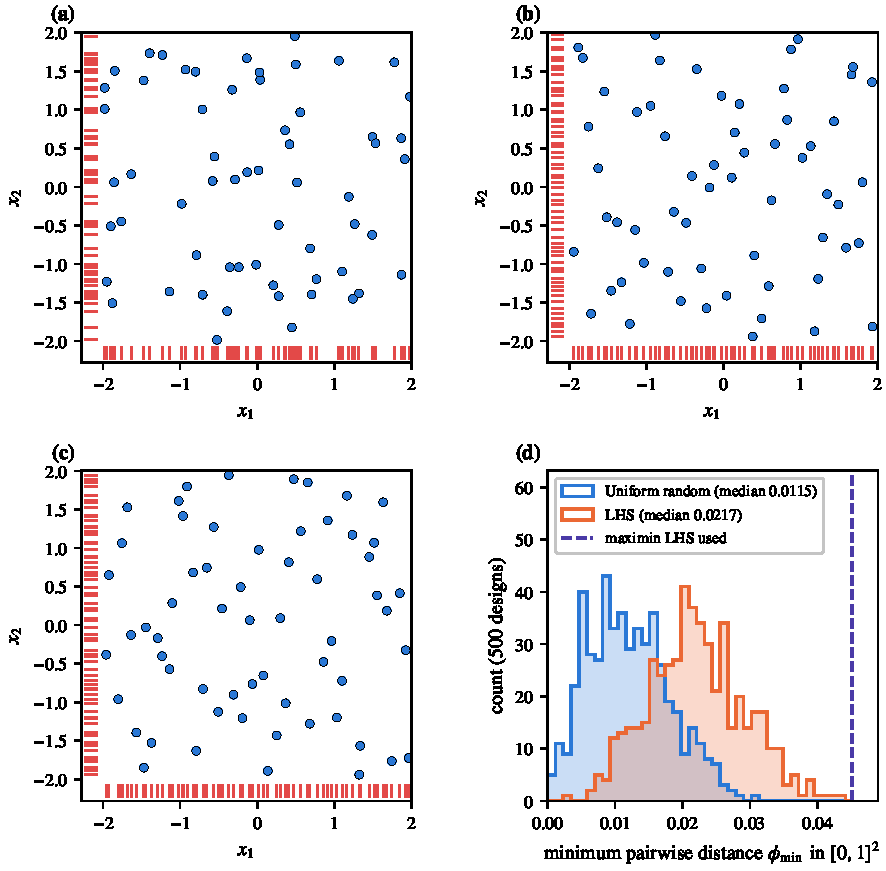
\includegraphics[width=0.86\textwidth]{rosenbrock/fig02_doe.pdf}
  \caption{Comparison of designs with the same budget $N=60$, shown in the Rosenbrock box. (a) Uniform random, $\phi_{\min}=0.0229$. (b) Latin hypercube, $\phi_{\min}=0.0251$. (c) Maximin LHS (best of 100 LHS draws), $\phi_{\min}=0.0452$, used for all results. Red ticks along the left and bottom edges are the one-dimensional projections of the points. (d) Distribution of $\phi_{\min}$, measured in the unit square, over 500 independent random and LHS designs; the dashed line is the maximin LHS actually used. The Trid study uses the same unit-square design scaled to $[-4,4]^2$.}
  \label{fig:doe}
\end{figure}

\begin{table}[!htbp]
  \centering
  \caption{Space-filling quality of the candidate designs, measured by the maximin distance $\phi_{\min}$ in the unit square ($N=60$, higher is better).}
  \label{tab:doe}
  \begin{adjustbox}{max width=\linewidth}
  \begin{tabular}{lccc}
    \toprule
    Design & $\phi_{\min}$ (seed 7) & Median over 500 draws & 5th percentile over 500 draws \\
    \midrule
    Uniform random & 0.0229 & 0.0115 & 0.0035 \\
    Latin hypercube & 0.0251 & 0.0217 & 0.0105 \\
    Maximin LHS (used) & 0.0452 & -- & -- \\
    \bottomrule
  \end{tabular}
  \end{adjustbox}
\end{table}

\subsection{Train/Test Split}

Figure~\ref{fig:R_split} shows the 45 training and 15 test points. The test points are spread over the whole box. Three lie on the valley floor, at $(-0.83,0.68)$, $(-0.46,0.22)$ and $(-0.10,0.06)$, where $f<3.4$. Two, $(0.91,1.36)$ and $(1.45,0.88)$, lie within 0.5 of the minimum but on the steep flanks ($f=27$ and 151), not in the low-$f$ valley near it, and one, $(-1.47,-1.85)$, approaches the corner $(-2,-2)$. Fifteen points cannot sample every feature, which is one reason CV and the dense-grid diagnostic are reported alongside the test metrics.

\begin{figure}[!htbp]
  \centering
  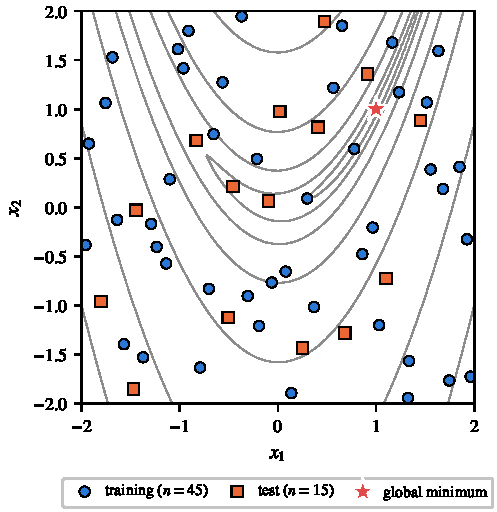
\includegraphics[width=0.5\textwidth]{rosenbrock/fig03_split.pdf}
  \caption{Rosenbrock: locations of the 45 training points and the 15 held-out test points over iso-lines of $f$; the star is the global minimum.}
  \label{fig:R_split}
\end{figure}

\subsection{Polynomial Degree Selection}\label{sec:tuning}

The degree sweep is shown in Fig.~\ref{fig:R_sweep} and listed in Table~\ref{tab:sweep}. For $p\le3$ the train, CV and test errors are all large (111 to 607) and close to one another: the model is too rigid and the error is bias, which more data would not remove. At $p=4$ every curve collapses by about 14 orders of magnitude to round-off ($\mathrm{RMSE}_{\mathrm{CV}}=1.27\times10^{-12}$), because the hypothesis space now contains the truth. The plain CV arg-min would have picked $p=5$, whose CV RMSE is lower by only $1.4\times10^{-13}$, a floating-point difference; the parsimony rule selects $p=4$, the true degree, from the data alone. The recovered physical coefficients match Eq.~\eqref{eq:rosen} to within $3.8\times10^{-13}$, and every coefficient that should vanish is below $2.5\times10^{-13}$.

Beyond $p=4$ no classic over-fitting appears in the \emph{train} or \emph{test} error: the data are noiseless and the truth is inside every larger space, so the extra coefficients are simply fitted as zero. What does appear is numerical. The condition number of the standardized design matrix grows from 33 at $p=4$ to $2.3\times10^3$ at $p=7$ and $2.1\times10^5$ at $p=8$, and the CV error climbs to $2.6\times10^{-11}$ at $p=7$ (36 terms on 36 fold points) and jumps to 82.9 at $p=8$. At $p=8$ each fold has 45 unknowns and 36 equations: the minimum-norm solution passes exactly through the fold's points but is not the true polynomial, and it is badly wrong on the left-out fold. On the full training set the same degree has a square $45\times45$ system whose unique solution is the truth again (test RMSE $1.9\times10^{-10}$). The gap between the CV curve and the train curve is therefore a signal of under-determination, not of noise-driven over-fitting.

\begin{figure}[!htbp]
  \centering
  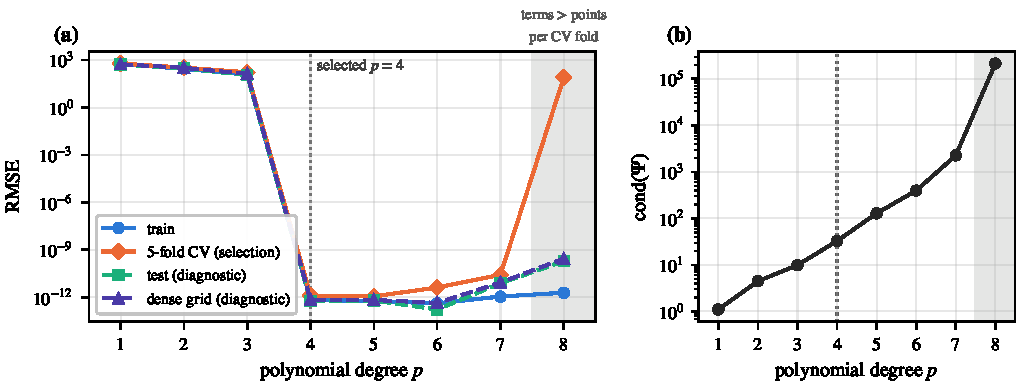
\includegraphics[width=\textwidth]{rosenbrock/fig04_degree_sweep.pdf}
  \caption{Rosenbrock: polynomial complexity study. (a) RMSE against degree $p$: training error, five-fold CV error on the training set (the only curve used for selection), and the held-out test and dense-grid errors added afterwards as diagnostics; the dotted line marks the selected $p=4$ and the shaded band marks degrees with more coefficients than points in a CV training fold. (b) Condition number of the standardized monomial design matrix.}
  \label{fig:R_sweep}
\end{figure}

\begin{table}[!htbp]
  \centering
  \caption{Polynomial degree sweep on the 45 training points: number of coefficients, condition number of the standardized design matrix, and five-fold CV RMSE for both functions. Selected degrees in bold.}
  \label{tab:sweep}
  \begin{adjustbox}{max width=\linewidth}
  \begin{tabular}{cccccc}
    \toprule
    $p$ & $n_{\mathrm{terms}}$ & Points per fold & cond$(\boldsymbol{\Psi})$ & CV RMSE, Rosenbrock & CV RMSE, Trid \\
    \midrule
    1 & 3 & 36 & 1.10 & $6.07\times10^{2}$ & $1.01\times10^{1}$ \\
    2 & 6 & 36 & 4.48 & $3.36\times10^{2}$ & $\mathbf{1.04\times10^{-14}}$ \\
    3 & 10 & 36 & 9.90 & $1.70\times10^{2}$ & $2.89\times10^{-14}$ \\
    4 & 15 & 36 & 32.6 & $\mathbf{1.27\times10^{-12}}$ & $1.82\times10^{-14}$ \\
    5 & 21 & 36 & 129 & $1.13\times10^{-12}$ & $2.58\times10^{-14}$ \\
    6 & 28 & 36 & 396 & $4.09\times10^{-12}$ & $3.37\times10^{-14}$ \\
    7 & 36 & 36 & $2.26\times10^{3}$ & $2.61\times10^{-11}$ & $5.56\times10^{-12}$ \\
    8 & 45 & 36 & $2.13\times10^{5}$ & $8.29\times10^{1}$ & $9.17\times10^{-1}$ \\
    \bottomrule
  \end{tabular}
  \end{adjustbox}
\end{table}

\subsection{Held-Out Validation and Cross-Validation}

Table~\ref{tab:test} lists the test metrics and Table~\ref{tab:cv} the CV and dense-grid errors; the parity plots are in Fig.~\ref{fig:R_parity}. All three models beat the mean baseline, whose $R^2$ is even negative ($-0.069$) because the test mean differs from the training mean. The polynomial is exact to round-off. The GP reaches a test RMSE of 0.0138 (NRMSE $7.8\times10^{-6}$) with a worst test error of 0.047. The cubic RBF has a test RMSE of 33.3 and a MaxAE of 116, but its $R^2=0.9962$ still looks excellent: the denominator of $R^2$ is the huge variance of the corner values, which is exactly why $R^2$ alone flatters a model on a function with this dynamic range.

The three error estimates in Table~\ref{tab:cv} do not agree, and the disagreement is informative. For the RBF the CV RMSE (78.2) is more than twice the test RMSE (33.3), and the dense grid (66.1) sits much closer to CV. The 15 test points happen to miss the worst errors, which lie in the corner itself and on the flanks, while CV predicts all 45 training points from models built on 36, which is more pessimistic but closer to the truth here. A single small test set can make a surrogate look better than it is, which is why CV and the error maps are needed alongside it.

\begin{table}[!htbp]
  \centering
  \caption{Held-out test metrics (15 points never used in fitting or selection). The range of $y_{\mathrm{test}}$ used for NRMSE is 1780.9 for Rosenbrock and 28.07 for Trid.}
  \label{tab:test}
  \begin{adjustbox}{max width=\linewidth}
  \begin{tabular}{llccccc}
    \toprule
    Function & Model & RMSE & MAE & $R^2$ & MaxAE & NRMSE \\
    \midrule
    \multirow{4}{*}{Rosenbrock} & Baseline, mean($y_{\mathrm{train}}$) & $558.4$ & $458.8$ & $-0.069$ & $1270.2$ & $0.314$ \\
     & Polynomial, $p=4$ & $5.87\times10^{-13}$ & $5.22\times10^{-13}$ & $1.000000$ & $8.98\times10^{-13}$ & $3.30\times10^{-16}$ \\
     & Cubic RBF & $33.27$ & $18.21$ & $0.996204$ & $115.55$ & $1.87\times10^{-2}$ \\
     & GP & $1.38\times10^{-2}$ & $7.48\times10^{-3}$ & $1.000000$ & $4.70\times10^{-2}$ & $7.75\times10^{-6}$ \\
    \midrule
    \multirow{4}{*}{Trid} & Baseline, mean($y_{\mathrm{train}}$) & $9.725$ & $8.375$ & $-0.262$ & $15.12$ & $0.347$ \\
     & Polynomial, $p=2$ & $7.91\times10^{-15}$ & $6.90\times10^{-15}$ & $1.000000$ & $1.55\times10^{-14}$ & $2.82\times10^{-16}$ \\
     & Cubic RBF & $4.25\times10^{-2}$ & $2.04\times10^{-2}$ & $0.999976$ & $0.155$ & $1.51\times10^{-3}$ \\
     & GP & $2.91\times10^{-5}$ & $1.87\times10^{-5}$ & $1.000000$ & $8.98\times10^{-5}$ & $1.04\times10^{-6}$ \\
    \bottomrule
  \end{tabular}
  \end{adjustbox}
\end{table}

\begin{table}[!htbp]
  \centering
  \caption{Five-fold CV RMSE on the training partition (used for selection), held-out test RMSE (final check), and dense-grid diagnostics over $14\,400$ points (available only because the truth is known). Grid NRMSE is normalized by the range of $f$ on the grid.}
  \label{tab:cv}
  \begin{adjustbox}{max width=\linewidth}
  \begin{tabular}{llccccc}
    \toprule
    Function & Model & CV RMSE & Test RMSE & Grid RMSE & Grid MaxAE & Grid NRMSE \\
    \midrule
    \multirow{3}{*}{Rosenbrock} & Polynomial, $p=4$ & $1.27\times10^{-12}$ & $5.87\times10^{-13}$ & $7.06\times10^{-13}$ & $3.13\times10^{-12}$ & $1.96\times10^{-16}$ \\
     & Cubic RBF & $78.24$ & $33.27$ & $66.12$ & $917.8$ & $1.83\times10^{-2}$ \\
     & GP & $5.78\times10^{-2}$ & $1.38\times10^{-2}$ & $3.27\times10^{-2}$ & $0.699$ & $9.06\times10^{-6}$ \\
    \midrule
    \multirow{3}{*}{Trid} & Polynomial, $p=2$ & $1.04\times10^{-14}$ & $7.91\times10^{-15}$ & $8.14\times10^{-15}$ & $2.84\times10^{-14}$ & $1.57\times10^{-16}$ \\
     & Cubic RBF & $0.178$ & $4.25\times10^{-2}$ & $0.156$ & $2.72$ & $2.99\times10^{-3}$ \\
     & GP & $4.69\times10^{-5}$ & $2.91\times10^{-5}$ & $5.58\times10^{-5}$ & $9.57\times10^{-4}$ & $1.07\times10^{-6}$ \\
    \bottomrule
  \end{tabular}
  \end{adjustbox}
\end{table}

\begin{figure}[!htbp]
  \centering
  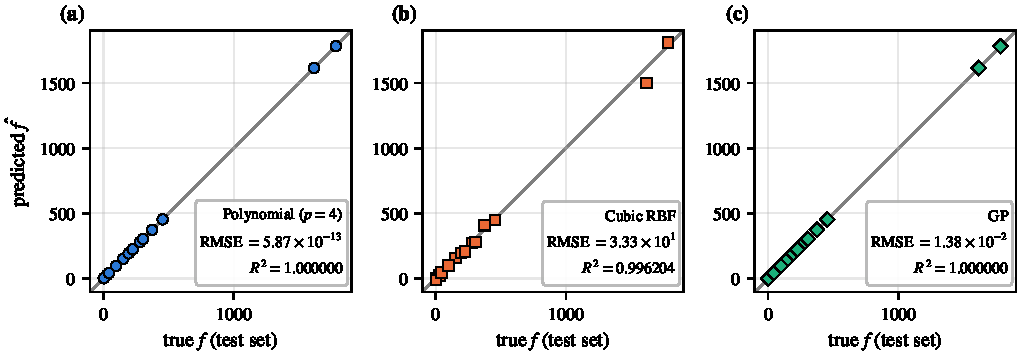
\includegraphics[width=\textwidth]{rosenbrock/fig05_parity.pdf}
  \caption{Rosenbrock: parity plots of predicted against true $f$ on the 15 held-out test points for (a) the degree-4 polynomial, (b) the cubic RBF and (c) the GP. The solid line is perfect prediction; the inset gives the test RMSE and $R^2$.}
  \label{fig:R_parity}
\end{figure}

\subsection{GP Hyperparameters and the Banana Valley}\label{sec:R_gp}

The fitted length scales are $\ell_1=2.57$ and $\ell_2=23.4$ in standardized units, or 3.11 and 27.4 in physical units. The ratio $\ell_2/\ell_1\approx8.8$ says that the function is roughly an order of magnitude more sensitive to $x_1$ than to $x_2$, which agrees with Eq.~\eqref{eq:rosen}: $x_1$ enters through the quartic $100x_1^4$ and the coupling $-200x_1^2x_2$, whereas $x_2$ enters only quadratically. The ARD kernel, however, measures sensitivity only along the coordinate axes. The valley is curved: inside the box it exists for $|x_1|\le\sqrt2$, and its tangent direction $(1,2x_1)$ rotates from $(1,-2.83)$ to $(1,2.83)$ along it, so no pair of axis-aligned length scales can describe ``slow along the valley, fast across it''. The two fitted values are a compromise averaged over the whole box, not a description of the valley.

The signal variance ended at its upper bound $\sigma_f^2=10^4$ and the noise variance close to its lower bound ($1.2\times10^{-12}$ against $10^{-12}$), and 3 of the 9 optimizer runs ended with an abnormal line-search termination; the run with the highest likelihood is kept. A stationary squared-exponential kernel approaches a polynomial only in the limit of large amplitude and long length scales~\cite{rasmussen2006}, so the likelihood keeps pushing $\sigma_f^2$ and $\ell_j$ upward, into a flat and poorly conditioned region. Table~\ref{tab:gpbound} shows that widening the bound does not settle the matter. With $\sigma_f^2\le10^6$ the likelihood rises to 214.7, but the training CV error gets worse (0.079 against 0.058). With $\sigma_f^2\le10^8$ the likelihood falls to 183.6, which cannot be the global optimum, because the $10^4$ solution is still admissible: the optimizer has found a different local optimum. The marginal likelihood is therefore multimodal and unreliable here, and the choice between the fits was made by training CV, which favors the $10^4$ bound. The bound acts as a mild regularizer. The principled remedy would be universal Kriging, a GP around a polynomial trend~\cite{forrester2008}, which is beyond the scope of this assignment.

\begin{table}[!htbp]
  \centering
  \caption{GP hyperparameters refitted with wider bounds on the normalized signal variance $\sigma_f^2$ (physical length scales). The alternatives are judged by training CV only; the first row of each block is the model used, for which 3 (Rosenbrock) and 8 (Trid) of the 9 optimizer runs ended with an abnormal line-search termination. A wider bound still admits the narrower optimum, so a lower likelihood indicates a different local optimum, not a worse model class.}
  \label{tab:gpbound}
  \begin{adjustbox}{max width=\linewidth}
  \begin{tabular}{llcccccc}
    \toprule
    Function & Bound on $\sigma_f^2$ & Fitted $\sigma_f^2$ & $\ell_1$ & $\ell_2$ & $\sigma_n^2$ & $\log p(\mathbf{y}\mid\boldsymbol{\theta})$ & CV RMSE \\
    \midrule
    \multirow{3}{*}{Rosenbrock} & $10^4$ (used) & $10^4$ (at bound) & 3.11 & 27.4 & $1.2\times10^{-12}$ & 197.8 & $5.78\times10^{-2}$ \\
     & $10^6$ & $10^6$ (at bound) & 4.80 & 99.8 & $9.8\times10^{-10}$ & 214.7 & $7.89\times10^{-2}$ \\
     & $10^8$ & $3.77\times10^{6}$ & 6.92 & 126.4 & $4.8\times10^{-8}$ & 183.6 & $6.10\times10^{-2}$ \\
    \midrule
    \multirow{3}{*}{Trid} & $10^4$ (used) & $10^4$ (at bound) & 37.5 & 37.2 & $1.9\times10^{-12}$ & 302.6 & $4.69\times10^{-5}$ \\
     & $10^6$ & $10^6$ (at bound) & 125.6 & 140.9 & $9.6\times10^{-9}$ & 260.1 & $2.74\times10^{-4}$ \\
     & $10^8$ & $1.14\times10^{5}$ & 48.8 & 51.8 & $6.7\times10^{-9}$ & 254.6 & $9.34\times10^{-5}$ \\
    \bottomrule
  \end{tabular}
  \end{adjustbox}
\end{table}

\subsection{Side-by-Side Visual Comparison}

Figures~\ref{fig:R_sbs_poly} to~\ref{fig:R_sbs_rbf} give the mandatory side-by-side comparison for the CV-best surrogate (the polynomial) and for the other two models; Fig.~\ref{fig:R_surf} gives the 3-D pair for the best surrogate. The polynomial error field (right panel of Fig.~\ref{fig:R_sbs_poly}) is pure round-off, at most $3.1\times10^{-12}$ against a signal of 3609. Its smooth large-scale pattern reflects floating-point cancellation in the quartic terms, not model error. Because this map carries no modeling information, the GP and RBF maps are where the failure patterns can be read. On every map of $f$ and $\hat f$ in this report, the color scale extends slightly below the minimum of $f$ on the grid (by 0.1\% of the range of $f$, i.e.\ to $-3.6$ for Rosenbrock and $-2.05$ for Trid), and surrogate values below that limit are drawn in red, so a clearly impossible prediction cannot hide in the darkest color.

For the GP (right panel of Fig.~\ref{fig:R_sbs_gp}) the error is below 0.05 almost everywhere and concentrates in the corner $(-2,-2)$, where it reaches 0.70. That corner combines the steepest part of the surface ($f=3609$) with the largest corner gap in the design: its nearest training point is 0.74 away, against 0.28 to 0.57 for the other three corners, and no point lies beyond the boundary to constrain the fit. For the RBF (right panel of Fig.~\ref{fig:R_sbs_rbf}) the error is three orders of magnitude larger and has the same hot spot, reaching 918 in the corner $(-2,-2)$. It also shows negative lobes of several hundred on both steep flanks near $(\pm1.7,-0.9)$, where the interpolant overshoots between samples, and the surrogate panel shows closed contours inside the valley that do not exist in the truth, enclosing a red region where $\hat f<-3.6$ and falls to $-16.8$, although $f\ge0$ everywhere. A cubic spline with a linear tail cannot reproduce a quartic, and near the boundary it relaxes toward its linear tail, whereas the true surface curves up fastest precisely at the edges~\cite{fornberg2002}. In all maps the largest errors sit in gaps between samples or outside the convex hull of the training points, never at the samples themselves.

\begin{figure}[!htbp]
  \centering
  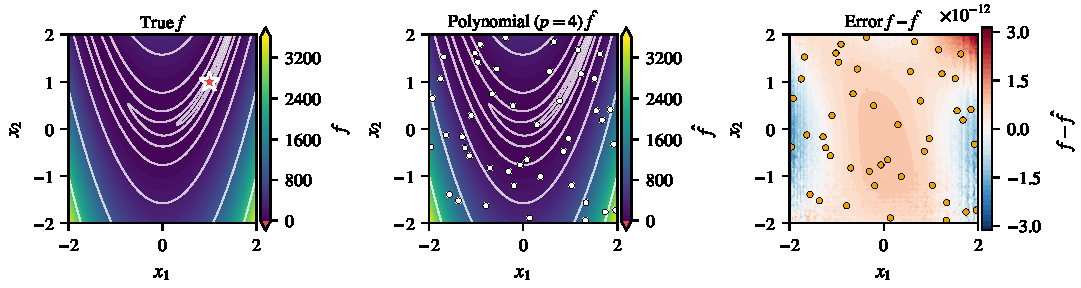
\includegraphics[width=\textwidth]{rosenbrock/fig06_side_by_side_poly.pdf}
  \caption{Rosenbrock, best surrogate by CV (degree-4 polynomial). Left: true $f$ on the $120\times120$ grid with the minimum marked. Center: surrogate $\hat f$ on the same grid with identical color limits, training points overlaid. Right: error $f-\hat f$ on a diverging scale centered at zero with training points overlaid; the maximum $|e|$ is $3.1\times10^{-12}$ (round-off). White iso-lines are drawn at the same levels in the first two panels.}
  \label{fig:R_sbs_poly}
\end{figure}

\begin{figure}[!htbp]
  \centering
  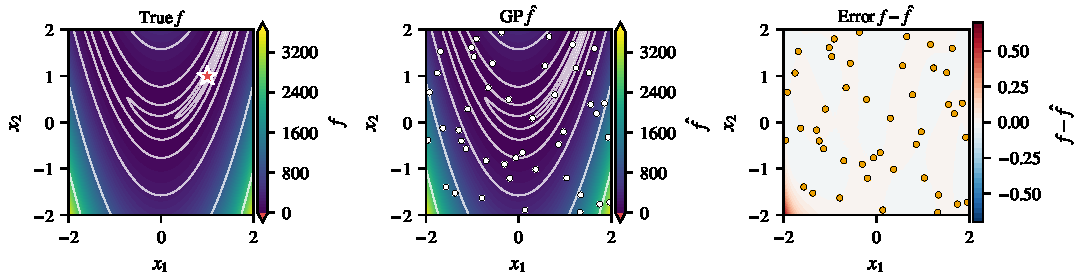
\includegraphics[width=\textwidth]{rosenbrock/fig06_side_by_side_gp.pdf}
  \caption{Rosenbrock, GP surrogate: true $f$, surrogate $\hat f$ with identical color limits, and error $f-\hat f$ (diverging scale centered at zero, maximum $|e|=0.699$ in the corner $(-2,-2)$), with training points overlaid on the surrogate and error panels.}
  \label{fig:R_sbs_gp}
\end{figure}

\begin{figure}[!htbp]
  \centering
  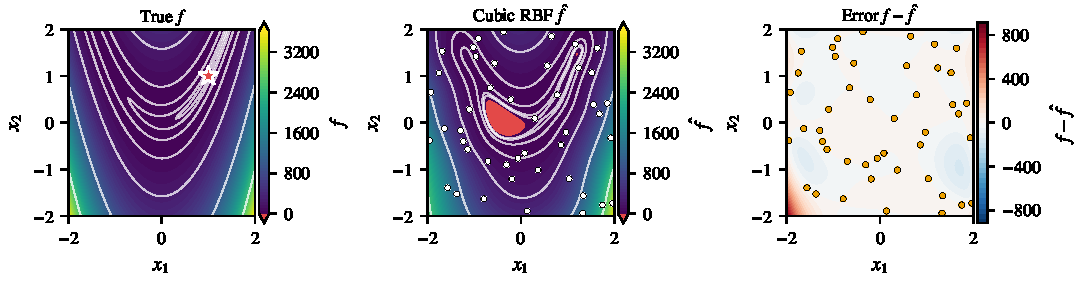
\includegraphics[width=\textwidth]{rosenbrock/fig06_side_by_side_rbf.pdf}
  \caption{Rosenbrock, cubic RBF surrogate: true $f$, surrogate $\hat f$ with identical color limits, and error $f-\hat f$ (diverging scale centered at zero, maximum $|e|=918$ in the corner $(-2,-2)$), with training points overlaid. Negative lobes on both steep flanks mark overshoot between samples. The red regions in the center panel are where the surrogate predicts values more than 0.1\% of the range of $f$ below its minimum ($\hat f<-3.6$): a large one reaching $-16.8$ inside closed contours that the truth does not have, and a small one near $(1.2,1.45)$ in the upper arm of the valley.}
  \label{fig:R_sbs_rbf}
\end{figure}

\begin{figure}[!htbp]
  \centering
  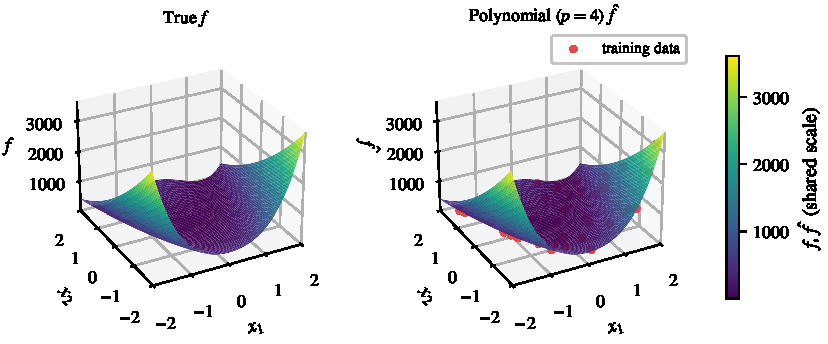
\includegraphics[width=0.95\textwidth]{rosenbrock/fig07_surfaces_poly.pdf}
  \caption{Rosenbrock: 3-D surfaces of the true function and of the degree-4 polynomial surrogate with identical axis limits, color limits and viewing angle; red dots are the training data.}
  \label{fig:R_surf}
\end{figure}

\subsection{Uncertainty Quantification}

Figure~\ref{fig:R_unc} compares the GP standard deviation $\hat\sigma$, which is available without knowing the truth, with the actual error $|f-\hat f|$, which is not. The two maps share their structure: both are smallest near the samples and largest in the corners, especially $(-2,-2)$. Over the grid, the Pearson correlation is 0.70 and the Spearman rank correlation 0.67, and 97.8\% of grid points satisfy $|f-\hat f|\le2\hat\sigma$. The 2.2\% outside the band matter most: they lie on the left side of the domain (centroid $(-1.50,-0.61)$) and include the worst error of all, 0.70, which exceeds twice the largest predicted standard deviation ($2\hat\sigma_{\max}=0.50$). The band therefore fails exactly where the error is largest. Away from the corners, $\hat\sigma$ is close to its numerical floor of $6.8\times10^{-3}$ (median $5.9\times10^{-3}$ in the central box, the same order as the value $7.0\times10^{-3}$ at the training points), so the useful information in $\hat\sigma$ lies in its rise toward the edges, up to 0.25. The two quantities are related because both grow with distance from the data. They are not the same quantity: $\hat\sigma$ depends only on the sample locations and the fitted kernel, not on the observed values at the prediction point, so it measures how poorly constrained the model is under its own assumptions, not how wrong it actually is. Panel~(c) shows this directly: at a given $\hat\sigma$ the true error spreads over two to three decades, and a lower branch of points has errors ten times smaller than $\hat\sigma$. The GP is a useful \emph{guide} to where to sample next, but not a certificate of accuracy.

\begin{figure}[!htbp]
  \centering
  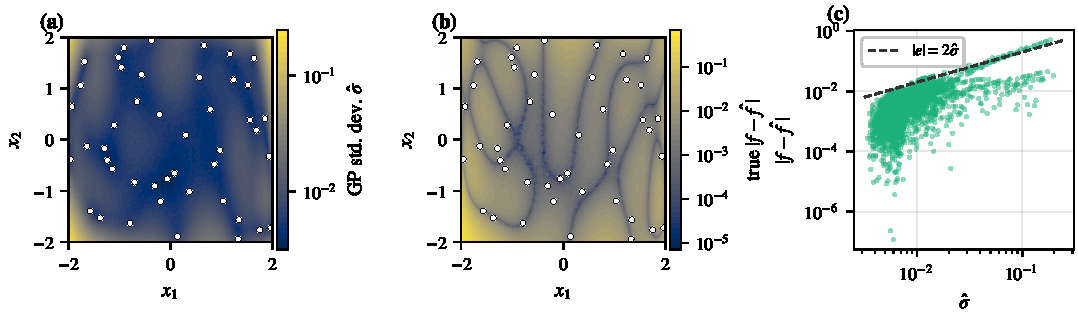
\includegraphics[width=\textwidth]{rosenbrock/fig08_gp_uncertainty.pdf}
  \caption{Rosenbrock, GP uncertainty. (a) Predicted standard deviation $\hat\sigma$ (log color scale), computable without the truth. (b) True absolute error $|f-\hat f|$ (log color scale). (c) $|f-\hat f|$ against $\hat\sigma$ for 3000 random grid points on logarithmic axes; the dashed line is $|e|=2\hat\sigma$. White dots in (a) and (b) are the training points.}
  \label{fig:R_unc}
\end{figure}

\subsection{Effect of Sample Size}\label{sec:R_learning}

The learning curves are shown in Fig.~\ref{fig:R_lc}. The polynomial stays at round-off ($\sim10^{-12}$) at every $N$, because 20 points already over-determine its 15 coefficients. The GP improves fastest, from a median grid RMSE of 2.91 at $N=20$ to 0.029 at $N=45$ and 0.0098 at $N=90$: going from 20 to 45 points buys a factor of 100, going from 45 to 90 only a factor of three. The RBF improves slowly, from 162 to 27.5 over the same range; in the central box it falls faster, from 61 to 3.8. Sampling variability is large at small $N$: at $N=30$ the five GP runs span a factor of 19 (0.093 to 1.79), which is a strong reason not to report a single-seed number as ``the'' accuracy of a model.

\begin{figure}[!htbp]
  \centering
  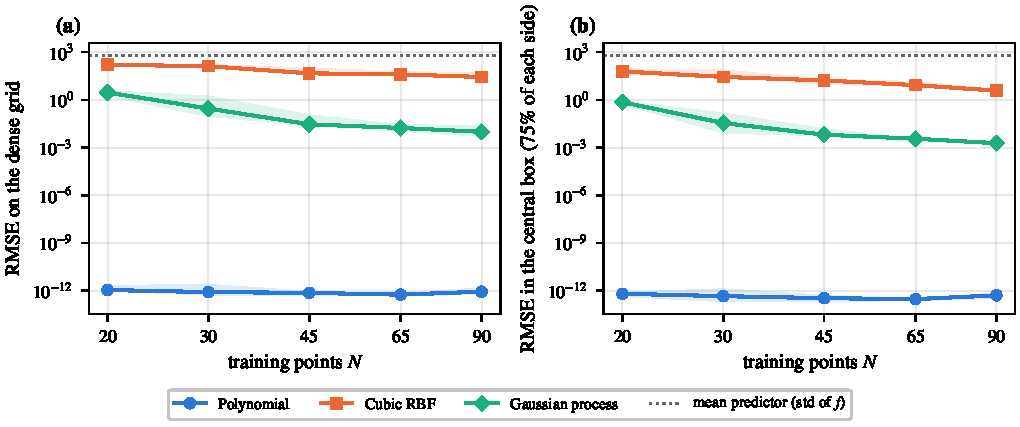
\includegraphics[width=\textwidth]{rosenbrock/fig09_learning_curve.pdf}
  \caption{Rosenbrock: learning curves on logarithmic axes. (a) RMSE over the full $120\times120$ grid. (b) RMSE over the central box whose sides are 75\% of the domain sides. Lines are medians over five independent LHS designs per training size and shaded bands span their minimum and maximum; the dotted line is the error of predicting the mean (standard deviation of $f$ on the grid, 624).}
  \label{fig:R_lc}
\end{figure}

\subsection{Surrogate-Based Optimization and Verification}

Table~\ref{tab:opt} and Fig.~\ref{fig:R_opt} give the optimization results. All 20 starts on the polynomial converge to $(1.000000,1.000000)$, and the true function there is $7.5\times10^{-16}$. All 20 starts on the GP converge to $(0.9940,0.9883)$, only 0.013 from the true minimum, with a true value of $4.5\times10^{-5}$ against a predicted $6.1\times10^{-4}$. The GP's positional error, $-0.0060$ in $x_1$ and $-0.0117$ in $x_2$, has a slope of 1.95. That is almost exactly the slope of the valley tangent, $2x_1=2$ at $x_1=1$. The surrogate found the valley, but not the precise point along its nearly flat floor, which is exactly the difficulty that makes Rosenbrock a benchmark.

The RBF shows why verification is not optional. Its best candidate, reached by 11 of the 20 starts, is a \emph{spurious} minimum at $(-0.44,0.04)$ with a predicted $\hat f=-16.8$: negative, although $f\ge0$ everywhere, and 1.73 away from the true minimum, where the true value is 4.50. It is an undershoot of the interpolant between samples inside the valley. The candidate closest to the truth, $(0.94,0.87)$ with $f=0.031$, ranks only second on the surrogate. Trusting the surrogate's own ranking would have picked the wrong design; one true evaluation per candidate, six in total, exposes the error. A second, small undershoot patch near $(1.2,1.45)$ ($\hat f<-3.6$, Fig.~\ref{fig:R_opt}b) was not reached by any start, so the multi-start search found four of at least five RBF minima, a reminder that 20 starts do not guarantee a complete search.

\begin{table}[!htbp]
  \centering
  \caption{Surrogate-based optimization (20 bounded Nelder--Mead starts per surrogate) and verification with the true function. ``Hits'' is the number of starts that ended in each cluster; $d$ is the distance to the known minimum. The last row of each block is the same multi-start search on the true function.}
  \label{tab:opt}
  \begin{adjustbox}{max width=\linewidth}
  \begin{tabular}{llcccccc}
    \toprule
    Function & Surrogate & Hits & $\hat{\mathbf{x}}^*$ & Predicted $\hat f(\hat{\mathbf{x}}^*)$ & True $f(\hat{\mathbf{x}}^*)$ & $|\hat f-f|$ & $d$ \\
    \midrule
    \multirow{7}{*}{Rosenbrock} & Polynomial & 20 & $(1.0000,\ 1.0000)$ & $-5.0\times10^{-13}$ & $7.5\times10^{-16}$ & $5.1\times10^{-13}$ & $2.1\times10^{-9}$ \\
     & RBF, cluster 1 & 11 & $(-0.4388,\ 0.0366)$ & $-16.77$ & $4.503$ & $21.27$ & $1.732$ \\
     & RBF, cluster 2 & 3 & $(0.9425,\ 0.8718)$ & $-1.761$ & $0.0307$ & $1.792$ & $0.140$ \\
     & RBF, cluster 3 & 3 & $(0.7209,\ 0.4026)$ & $-0.797$ & $1.449$ & $2.247$ & $0.659$ \\
     & RBF, cluster 4 & 3 & $(-1.1492,\ 1.3781)$ & $8.312$ & $4.948$ & $3.364$ & $2.182$ \\
     & GP & 20 & $(0.9940,\ 0.9883)$ & $6.1\times10^{-4}$ & $4.5\times10^{-5}$ & $5.7\times10^{-4}$ & $1.3\times10^{-2}$ \\
     & True $f$ (check) & 20 & $(1.0000,\ 1.0000)$ & -- & $1.9\times10^{-20}$ & -- & $2.6\times10^{-10}$ \\
    \midrule
    \multirow{4}{*}{Trid} & Polynomial & 20 & $(2.0000,\ 2.0000)$ & $-2.000000$ & $-2.000000$ & $1.3\times10^{-14}$ & $1.0\times10^{-8}$ \\
     & RBF & 20 & $(1.9950,\ 1.9933)$ & $-2.012319$ & $-1.999964$ & $1.2\times10^{-2}$ & $8.4\times10^{-3}$ \\
     & GP & 20 & $(1.9995,\ 1.9997)$ & $-2.000000$ & $-2.000000$ & $2.7\times10^{-7}$ & $5.7\times10^{-4}$ \\
     & True $f$ (check) & 20 & $(2.0000,\ 2.0000)$ & -- & $-2.000000$ & -- & $1.1\times10^{-8}$ \\
    \bottomrule
  \end{tabular}
  \end{adjustbox}
\end{table}

\begin{figure}[!htbp]
  \centering
  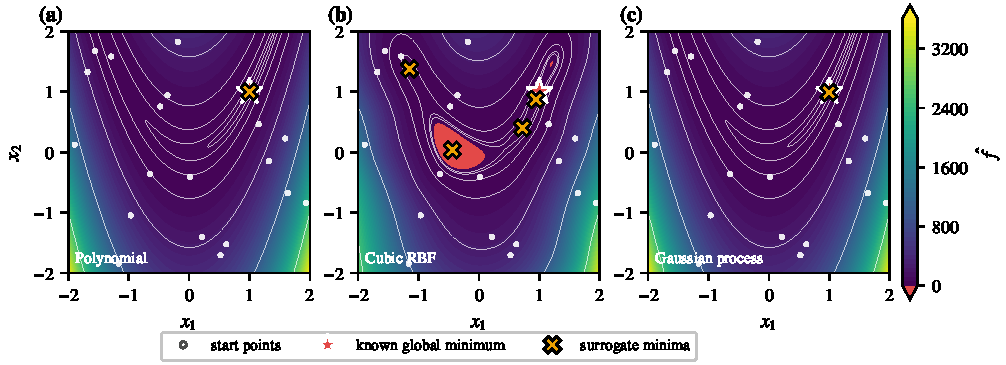
\includegraphics[width=\textwidth]{rosenbrock/fig10_optimisation.pdf}
  \caption{Rosenbrock: multi-start optimization on (a) the degree-4 polynomial, (b) the cubic RBF and (c) the GP. The background is each surrogate $\hat f$ with the color limits of the true function and white iso-lines of $\hat f$; white dots are the 20 start points, crosses the distinct surrogate minima, and the star the known global minimum. Four distinct RBF minima were found from the 20 starts, including the spurious deepest one at $(-0.44,0.04)$, which lies inside the large red region where $\hat f<-3.6$. The small red patch near $(1.2,1.45)$ is a further undershoot that no start reached.}
  \label{fig:R_opt}
\end{figure}

\subsection{Extrapolation}

Table~\ref{tab:extrap} and Fig.~\ref{fig:R_extrap} give the reduced-box experiment (training on $[-1,1]^2$). Inside the box the GP error is small (RMSE 0.0064); outside it rises to 14.9, a factor of 2320, with a worst error of 121 in the corners, where the true function reaches 3609 but the GP has no data to follow the quartic growth. The RBF, whose linear tail extrapolates linearly, is worse in absolute terms (574 outside). The polynomial stays exact outside the box, but only because its assumed form happens to be the true one. In a real problem that is unknowable, and a surrogate should never be trusted outside its training box. Note also that the true minimum $(1,1)$ lies on the corner of this training box, so any optimizer that stops at the edge of the DOE box is telling the engineer to re-sample, not to trust the answer.

\begin{table}[!htbp]
  \centering
  \caption{Extrapolation test: each model is trained on 45 LHS points in the central sub-box ($[-1,1]^2$ for Rosenbrock, $[-2,2]^2$ for Trid) and evaluated over the full grid. The last column is the ratio of the RMSE outside to the RMSE inside the training box.}
  \label{tab:extrap}
  \begin{adjustbox}{max width=\linewidth}
  \begin{tabular}{llccccc}
    \toprule
    Function & Model & RMSE inside & RMSE outside & MaxAE inside & MaxAE outside & Ratio out/in \\
    \midrule
    \multirow{3}{*}{Rosenbrock} & Polynomial & $5.9\times10^{-14}$ & $8.3\times10^{-13}$ & $2.0\times10^{-13}$ & $3.6\times10^{-12}$ & 14 \\
     & Cubic RBF & $6.07$ & $574.2$ & $66.4$ & $2622$ & 95 \\
     & GP & $6.4\times10^{-3}$ & $14.93$ & $0.101$ & $120.6$ & 2321 \\
    \midrule
    \multirow{3}{*}{Trid} & Polynomial & $2.8\times10^{-15}$ & $1.2\times10^{-14}$ & $8.9\times10^{-15}$ & $4.3\times10^{-14}$ & 4.4 \\
     & Cubic RBF & $5.3\times10^{-2}$ & $3.712$ & $0.831$ & $19.12$ & 70 \\
     & GP & $9.9\times10^{-6}$ & $2.8\times10^{-3}$ & $1.7\times10^{-4}$ & $2.6\times10^{-2}$ & 287 \\
    \bottomrule
  \end{tabular}
  \end{adjustbox}
\end{table}

\begin{figure}[!htbp]
  \centering
  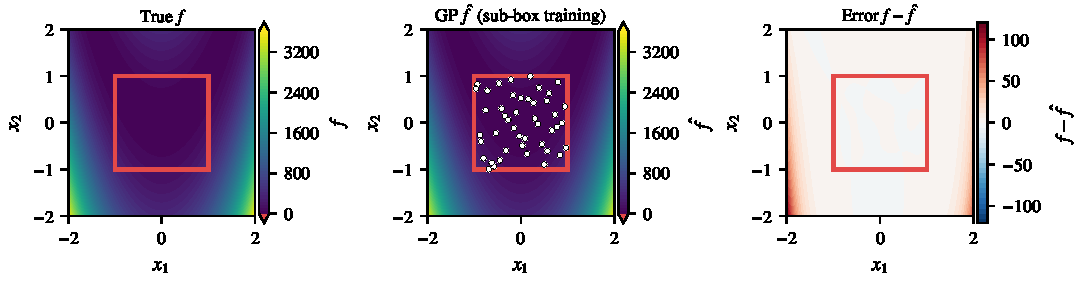
\includegraphics[width=\textwidth]{rosenbrock/fig11_extrapolation_gp.pdf}
  \caption{Rosenbrock, extrapolation of a GP trained only inside the red box $[-1,1]^2$ (white dots). Left: true $f$. Center: GP prediction over the full domain with the color limits of the true function (values above them saturate; no value falls below the red undershoot limit). Right: error $f-\hat f$, which grows by three orders of magnitude outside the training box.}
  \label{fig:R_extrap}
\end{figure}

% ---------------------------------------------------------------------
\section{Results, Part B: Trid Function}\label{sec:trid}

\subsection{Function, Domain and Analytical Minimum}

The two-variable Trid function, Eq.~\eqref{eq:trid}, is shown in Fig.~\ref{fig:T_truth}. Its minimum can be found by hand. Setting the gradient to zero,
\begin{equation}
  \nabla f=\begin{bmatrix}2(x_1-1)-x_2\\2(x_2-1)-x_1\end{bmatrix}=\mathbf{0}
  \quad\Longrightarrow\quad
  \underbrace{\begin{bmatrix}2&-1\\-1&2\end{bmatrix}}_{\mathbf{H}}\begin{bmatrix}x_1\\x_2\end{bmatrix}=\begin{bmatrix}2\\2\end{bmatrix}.
  \label{eq:trid_grad}
\end{equation}
Adding the two equations gives $x_1+x_2=4$; subtracting them gives $3(x_1-x_2)=0$. Hence
\begin{equation}
  \mathbf{x}^*=(2,\,2),\qquad f(\mathbf{x}^*)=(2-1)^2+(2-1)^2-2\cdot2=-2 .
  \label{eq:trid_min}
\end{equation}
The Hessian $\mathbf{H}$ is constant, with eigenvalues 1 and 3 and eigenvectors along $(1,1)$ and $(1,-1)$. It is positive definite, so $f$ is strictly convex and $(2,2)$ is its unique global minimum on any domain containing it. The level sets are ellipses tilted at $45^\circ$ with axis ratio $\sqrt3$, elongated along $(1,1)$, the direction of the smaller eigenvalue (Fig.~\ref{fig:T_truth}a). On $[-4,4]^2$ the function ranges from $-2$ to 50, the maximum occurring at the corners $(-4,4)$ and $(4,-4)$, where the cross term $-x_1x_2$ is largest and positive.

\begin{figure}[!htbp]
  \centering
  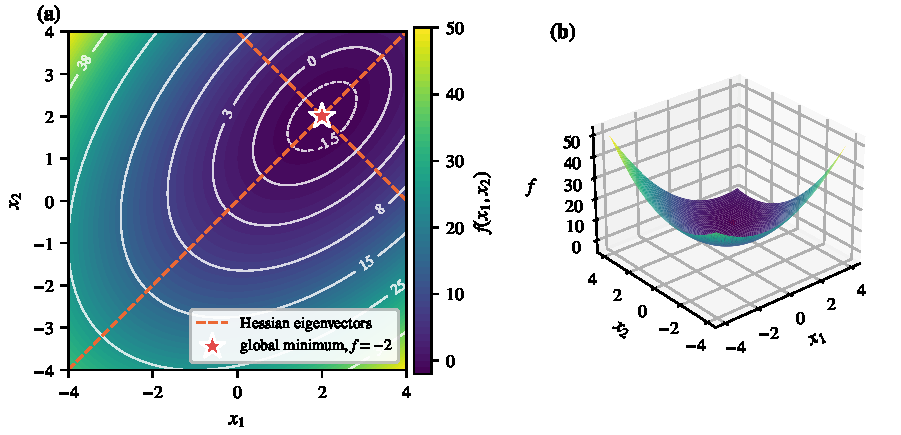
\includegraphics[width=\textwidth]{trid/fig01_truth.pdf}
  \caption{Trid function on $[-4,4]^2$. (a) Filled contour map with iso-lines at $f=-1.5,0,3,8,15,25,38$; dashed lines are the Hessian eigenvector directions $(1,1)$ and $(1,-1)$ through the minimum, and the star is the global minimum $f=-2$ at $(2,2)$. (b) Three-dimensional surface with the minimum marked.}
  \label{fig:T_truth}
\end{figure}

\subsection{Design of Experiments and Split}

The Trid study uses the same maximin LHS as Part~A (Fig.~\ref{fig:doe}c and Table~\ref{tab:doe}), scaled to $[-4,4]^2$. Its $\phi_{\min}=0.0452$ in unit coordinates corresponds to 0.36 in physical units, and the characteristic spacing $\sqrt{|\mathcal{X}|/n}$ of the 45 training points is 1.19. That spacing is adequate here because the Trid function has no short-wavelength features: its curvature is constant, and a quadratic is fully determined by six well-placed values. The same argument justifies $N=60$: ten times the six coefficients of the exact model, with 36 points per CV fold. The split is shown in Fig.~\ref{fig:T_split}; the test points cover all four quadrants, and two of them, $(1.83,2.72)$ and $(2.91,1.77)$, lie 0.74 and 0.94 from the minimum.

\begin{figure}[!htbp]
  \centering
  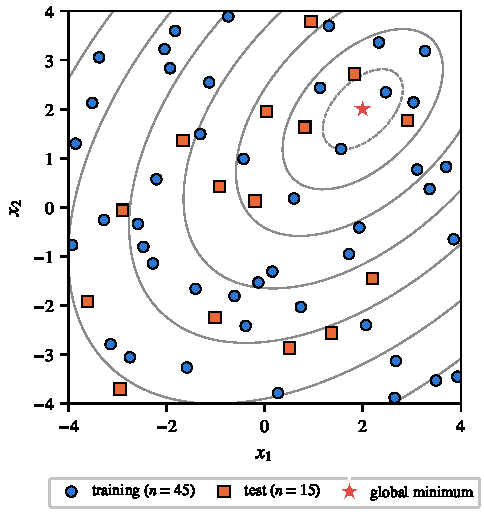
\includegraphics[width=0.5\textwidth]{trid/fig03_split.pdf}
  \caption{Trid: locations of the 45 training points and the 15 held-out test points over iso-lines of $f$; the star is the global minimum.}
  \label{fig:T_split}
\end{figure}

\subsection{Polynomial Degree Selection}

The Trid degree sweep (Fig.~\ref{fig:T_sweep}, Table~\ref{tab:sweep}) repeats the Rosenbrock pattern at a lower degree. Degree 1 under-fits: a plane cannot represent a bowl, and its train, CV and test RMSE (9.68, 10.1 and 6.22) are almost equal to the spread of the data itself, a pure bias error. At $p=2$ the CV RMSE drops to $1.04\times10^{-14}$, 15 orders of magnitude lower, and the parsimony rule selects the true degree. Degrees 3 to 6 stay at round-off, degree 7 rises to $5.6\times10^{-12}$ with the condition number, and degree 8 jumps to 0.92 because the folds are under-determined, as explained for Part~A. The recovered physical coefficients match Eq.~\eqref{eq:trid} to within $1.2\times10^{-14}$. Solving $\nabla\hat f=\mathbf{0}$ for the \emph{fitted} quadratic gives a stationary point that differs from $(2,2)$ by $1.0\times10^{-14}$ in $x_1$ and $5\times10^{-15}$ in $x_2$, and a Hessian equal to $\mathbf{H}$ of Eq.~\eqref{eq:trid_grad} to within $4\times10^{-15}$, reproducing the hand derivation of Eq.~\eqref{eq:trid_min} from the surrogate itself.

\begin{figure}[!htbp]
  \centering
  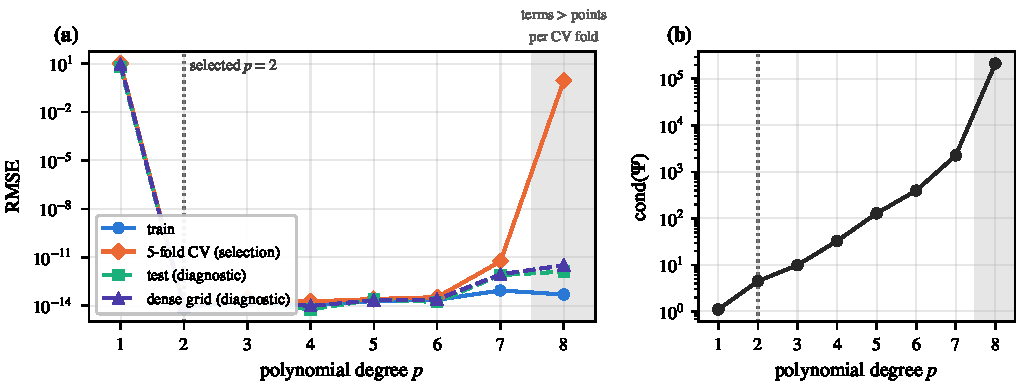
\includegraphics[width=\textwidth]{trid/fig04_degree_sweep.pdf}
  \caption{Trid: polynomial complexity study. (a) Training, five-fold CV (selection) and test and dense-grid (diagnostic) RMSE against degree; the dotted line marks the selected $p=2$ and the shaded band marks degrees with more coefficients than points per CV fold. (b) Condition number of the standardized design matrix.}
  \label{fig:T_sweep}
\end{figure}

\subsection{Held-Out Validation, Cross-Validation and GP Hyperparameters}

The Trid metrics are in Tables~\ref{tab:test} and~\ref{tab:cv}, and the parity plots in Fig.~\ref{fig:T_parity}. All models beat the baseline (test RMSE 9.73, $R^2=-0.26$). The polynomial is exact to $7.9\times10^{-15}$; the GP reaches $2.9\times10^{-5}$ (NRMSE $1.0\times10^{-6}$); and the RBF reaches 0.042 (NRMSE $1.5\times10^{-3}$) with a test MaxAE of 0.155. As for Rosenbrock, the RBF test RMSE underestimates the grid RMSE (0.156) by a factor of almost four, while CV (0.178) is close to it.

The GP length scales are 37.5 and 37.2 in physical units (Table~\ref{tab:gpbound}), almost identical and about 4.7 times the box width. Equal length scales are expected: the Trid function is symmetric under $x_1\leftrightarrow x_2$ and so is the design box. Their size says that the response is low-order and smooth relative to the domain, so the GP is effectively modeling a polynomial-like trend. As for Rosenbrock, the signal variance sits at its upper bound and the noise variance near its lower bound ($1.9\times10^{-12}$); here 8 of the 9 optimizer runs ended abnormally. Widening the bound gave lower likelihoods (260.1 and 254.6 against 302.6), which again reveals other local optima rather than better models, and worse CV errors (Table~\ref{tab:gpbound}), so the $10^4$ bound was kept for the reason given in Sec.~\ref{sec:R_gp}.

\begin{figure}[!htbp]
  \centering
  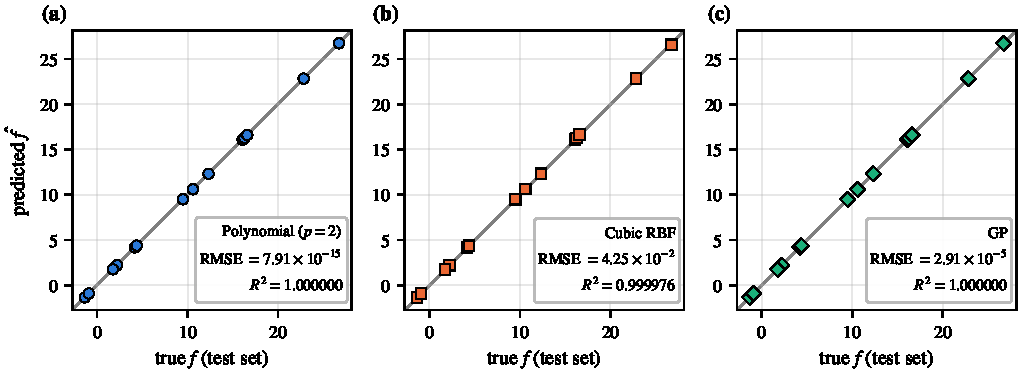
\includegraphics[width=\textwidth]{trid/fig05_parity.pdf}
  \caption{Trid: parity plots on the 15 held-out test points for (a) the degree-2 polynomial, (b) the cubic RBF and (c) the GP, with test RMSE and $R^2$ in the insets.}
  \label{fig:T_parity}
\end{figure}

\subsection{Side-by-Side Visual Comparison}

The side-by-side comparisons are in Figs.~\ref{fig:T_sbs_poly} to~\ref{fig:T_sbs_rbf}, and the 3-D pair of the best surrogate in Fig.~\ref{fig:T_surf}. The polynomial error is round-off ($2.8\times10^{-14}$). The GP error (Fig.~\ref{fig:T_sbs_gp}) is below $10^{-4}$ in the interior and peaks at $9.6\times10^{-4}$ at the edges and corners. The RBF error (Fig.~\ref{fig:T_sbs_rbf}) is the clearest failure pattern of the whole study: it is small inside the sampled region (the learning curve of Fig.~\ref{fig:T_lc} gives a central-box RMSE of about 0.03 at $N=45$) and grows sharply toward the boundary, reaching 2.72 in the corner $(-4,4)$. The Trid function has constant curvature everywhere; the cubic RBF with a linear tail cannot represent a quadratic exactly, and near the boundary, where no samples lie beyond, it relaxes toward its linear tail and loses the curvature~\cite{fornberg2002}. The error is therefore largest precisely where the true surface is steepest and the data give no support from outside.

\begin{figure}[!htbp]
  \centering
  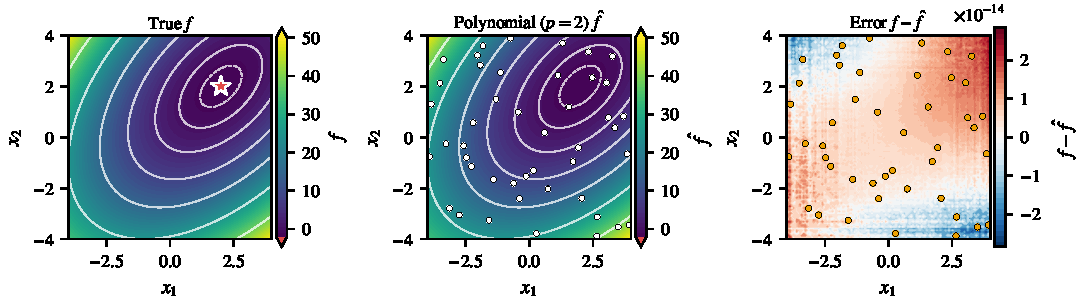
\includegraphics[width=\textwidth]{trid/fig06_side_by_side_poly.pdf}
  \caption{Trid, best surrogate by CV (degree-2 polynomial): true $f$, surrogate $\hat f$ with identical color limits and training points, and error $f-\hat f$ on a diverging scale centered at zero with training points (maximum $|e|=2.8\times10^{-14}$, round-off).}
  \label{fig:T_sbs_poly}
\end{figure}

\begin{figure}[!htbp]
  \centering
  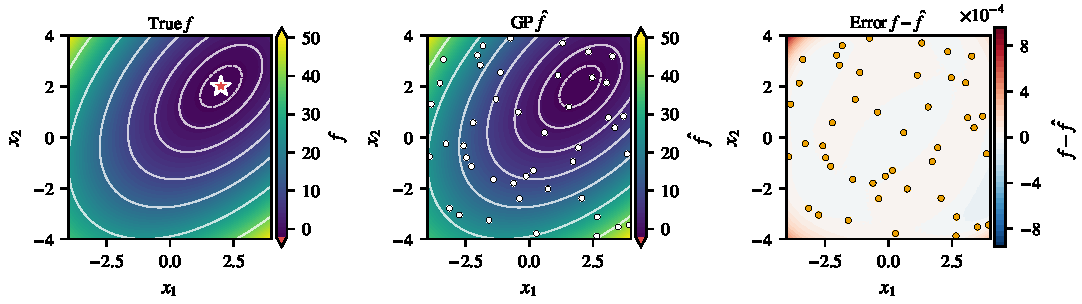
\includegraphics[width=\textwidth]{trid/fig06_side_by_side_gp.pdf}
  \caption{Trid, GP surrogate: true $f$, surrogate $\hat f$ with identical color limits, and error $f-\hat f$ (diverging scale centered at zero, maximum $|e|=9.6\times10^{-4}$), with training points overlaid.}
  \label{fig:T_sbs_gp}
\end{figure}

\begin{figure}[!htbp]
  \centering
  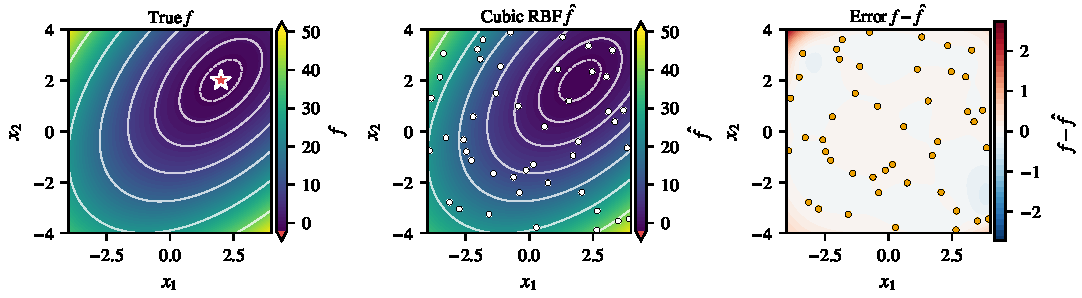
\includegraphics[width=\textwidth]{trid/fig06_side_by_side_rbf.pdf}
  \caption{Trid, cubic RBF surrogate: true $f$, surrogate $\hat f$ with identical color limits, and error $f-\hat f$ (diverging scale centered at zero, maximum $|e|=2.72$ in the corner $(-4,4)$), with training points overlaid. The error is confined to a band along the boundary.}
  \label{fig:T_sbs_rbf}
\end{figure}

\begin{figure}[!htbp]
  \centering
  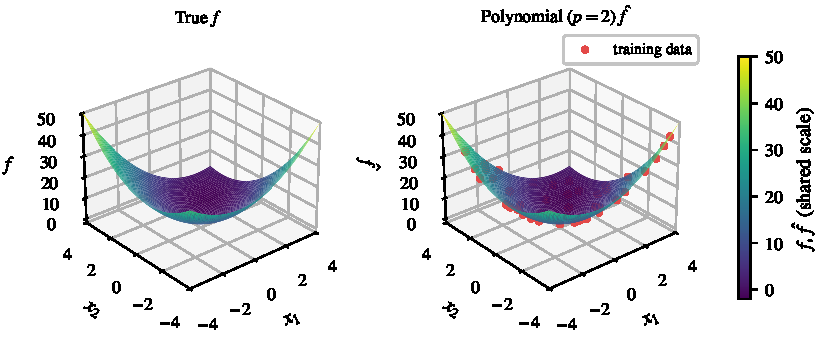
\includegraphics[width=0.95\textwidth]{trid/fig07_surfaces_poly.pdf}
  \caption{Trid: 3-D surfaces of the true function and of the degree-2 polynomial surrogate with identical axis limits, color limits and viewing angle; red dots are the training data.}
  \label{fig:T_surf}
\end{figure}

\subsection{Uncertainty Quantification}

For the Trid GP (Fig.~\ref{fig:T_unc}), $\hat\sigma$ is again smallest near the samples and largest at the edges and corners. Every grid point satisfies $|f-\hat f|\le2\hat\sigma$, so the uncertainty band is conservative. The Pearson correlation is 0.68, but the Spearman rank correlation is only 0.27. The reason is visible in panel~(b): in the interior the true error is at the level of $10^{-5}$ to $10^{-8}$ and forms thin curved bands where $f-\hat f$ changes sign, a structure that has nothing to do with distance from the data. $\hat\sigma$ tracks the large errors at the edges (hence the reasonable Pearson value), but in the interior it is itself at its numerical floor: its median over the central box, $7.5\times10^{-5}$, is of the same order as the floor $\sqrt{\alpha+\sigma_n^2}\,\mathrm{std}(y_{\mathrm{train}})=1.2\times10^{-4}$ and as its value at the training points, $1.1\times10^{-4}$. Both $\hat\sigma$ and the true error are therefore dominated by numerical effects there, and one cannot rank the other. A rerun of the same script with the same package versions on a Linux machine confirms this: every other result in this report agrees within 1\%, but the Trid correlations change to 0.20 (Spearman) and 0.65 (Pearson), because they are computed from quantities at round-off level. This is a clear illustration that $\hat\sigma$ is a statement about the model's assumptions and the sample geometry, not a measurement of the actual error.

\begin{figure}[!htbp]
  \centering
  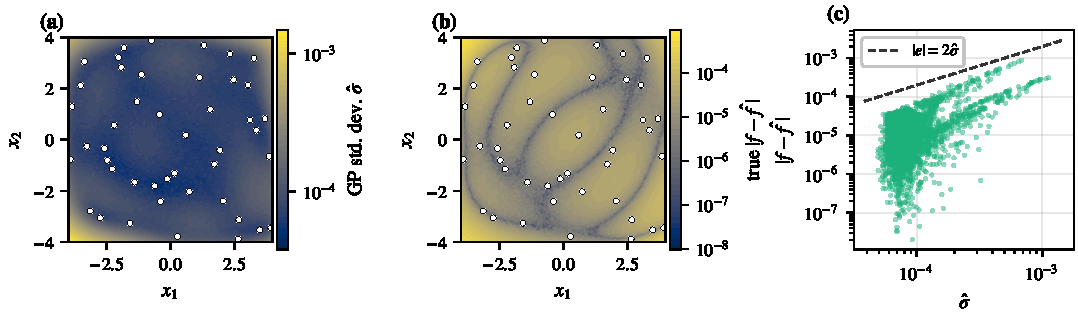
\includegraphics[width=\textwidth]{trid/fig08_gp_uncertainty.pdf}
  \caption{Trid, GP uncertainty. (a) Predicted standard deviation $\hat\sigma$ and (b) true absolute error $|f-\hat f|$, both on log color scales with the training points. (c) $|f-\hat f|$ against $\hat\sigma$ for 3000 random grid points; every point lies below the line $|e|=2\hat\sigma$.}
  \label{fig:T_unc}
\end{figure}

\subsection{Effect of Sample Size}

The Trid learning curves (Fig.~\ref{fig:T_lc}) separate interior from edge behavior. In the central box the RBF error falls steadily with $N$, from 0.235 to 0.0094, as a converging interpolant should. Over the full grid, however, its median RMSE stops falling after $N=45$ (0.091, then 0.110 at $N=65$ and 0.177 at $N=90$). With five draws per size the ranges overlap (0.069 to 0.218 at $N=45$, 0.117 to 0.265 at $N=90$), so the rise itself is not significant, but the stagnation against a falling core error is clear. The median condition number of the saddle-point system grows from $1.0\times10^4$ at $N=20$ to $2.2\times10^6$ at $N=90$, far from causing round-off trouble in double precision, so conditioning is not the explanation. A plausible one is the boundary behavior of polyharmonic splines~\cite{fornberg2002}: added interior points improve the interior but do little for the loss of curvature in the edge band, which dominates the full-grid error. The GP shows the same pattern at a much lower level: its full-grid median rises slightly (from $4.8\times10^{-5}$ at $N=45$ to $7.0\times10^{-5}$ at $N=90$) while its core error settles at about $1.7\times10^{-5}$. That floor is most likely set by the near-degenerate kernel (very long length scales and a noise variance near $10^{-12}$), not by the amount of data. The polynomial is at round-off for every $N$.

\begin{figure}[!htbp]
  \centering
  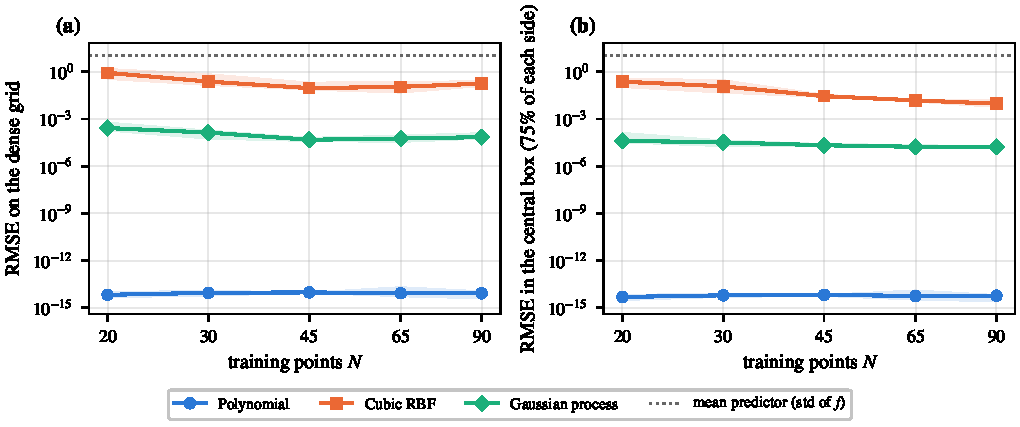
\includegraphics[width=\textwidth]{trid/fig09_learning_curve.pdf}
  \caption{Trid: learning curves on logarithmic axes. (a) RMSE over the full grid. (b) RMSE over the central box whose sides are 75\% of the domain sides. Lines are medians over five LHS designs per size and bands their range; the dotted line is the error of predicting the mean (standard deviation of $f$, 10.9). Beyond $N=45$ the full-grid RBF and GP errors stop falling, while their core errors do not rise.}
  \label{fig:T_lc}
\end{figure}

\subsection{Surrogate-Based Optimization and Verification}

All three surrogates lead every one of the 20 starts to a single minimum (Table~\ref{tab:opt} and Fig.~\ref{fig:T_opt}). The polynomial minimum lies $1.0\times10^{-8}$ from $(2,2)$, a distance set by the Nelder--Mead tolerance, with a true value of $-2.000000$. The GP minimum is 0.00057 from $(2,2)$ and its true value, $-1.9999998$, agrees with the prediction to $2.7\times10^{-7}$. The RBF minimum is 0.0084 from $(2,2)$, and it predicts $\hat f=-2.0123$, a value \emph{lower} than the true global minimum $-2$: the surrogate promises a design better than any design that exists. The true value at its point, $-1.99996$, is still within $3.6\times10^{-5}$ of the optimum, so for this convex function the positional error is harmless, but the predicted performance is optimistic. The multi-start search on the true function returns $(2,2)$ and $f=-2$, confirming the hand derivation of Eq.~\eqref{eq:trid_min} numerically. The analytical solution, the stationary point of the fitted quadratic and the numerical searches all agree.

\begin{figure}[!htbp]
  \centering
  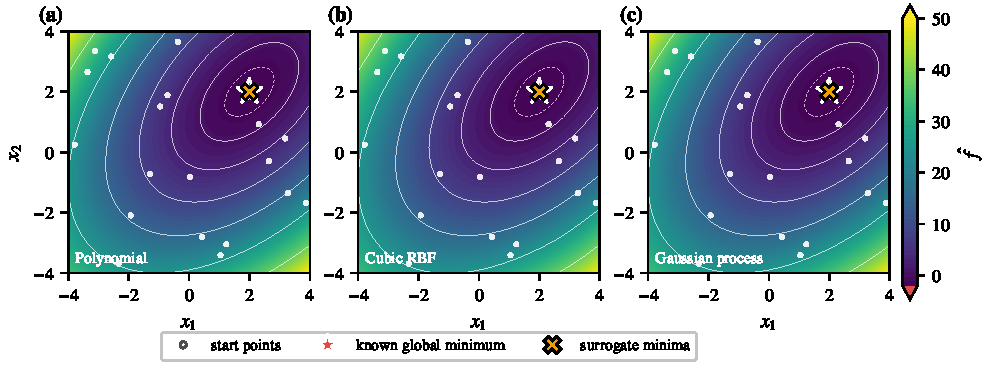
\includegraphics[width=\textwidth]{trid/fig10_optimisation.pdf}
  \caption{Trid: multi-start optimization on (a) the degree-2 polynomial, (b) the cubic RBF and (c) the GP, drawn over each surrogate with the color limits of the true function; white dots are the 20 start points, crosses the surrogate minima and the star the known global minimum at $(2,2)$.}
  \label{fig:T_opt}
\end{figure}

\subsection{Extrapolation}

Trained on $[-2,2]^2$, which has the minimum $(2,2)$ at its corner, the GP error rises from $9.9\times10^{-6}$ inside to $2.8\times10^{-3}$ outside, a factor of 287 (Table~\ref{tab:extrap} and Fig.~\ref{fig:T_extrap}). The ratio is smaller than for Rosenbrock because the Trid function keeps the same quadratic shape everywhere, so the long-length-scale GP continues the trend reasonably well. The RBF error grows by a factor of 70, to 19 at the corners, because its linear tail cannot follow the quadratic growth. The polynomial again extrapolates exactly, for the same reason as in Part~A.

\begin{figure}[!htbp]
  \centering
  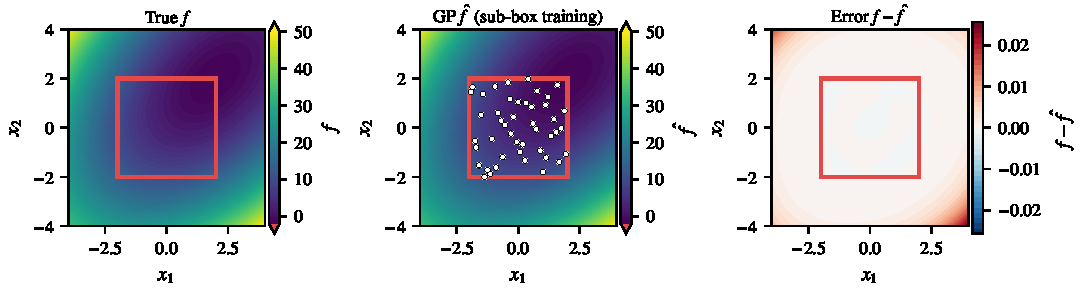
\includegraphics[width=\textwidth]{trid/fig11_extrapolation_gp.pdf}
  \caption{Trid, extrapolation of a GP trained only inside the red box $[-2,2]^2$ (white dots): true $f$, GP prediction with the color limits of the true function, and error $f-\hat f$, which grows toward the corners of the full domain.}
  \label{fig:T_extrap}
\end{figure}

\subsection{Evaluation Budget}

Table~\ref{tab:budget} separates the main DOE budget from the extra evaluations made only because the truth is cheap. Only the 60 DOE runs and the verification runs would exist in a real project; the grid, learning-curve, reduced-box and true-function multi-start evaluations are teaching diagnostics and were never used for fitting or selection.

\begin{table}[!htbp]
  \centering
  \caption{Accounting of true-function evaluations. Only the first two rows would be spent in a real study.}
  \label{tab:budget}
  \begin{adjustbox}{max width=\linewidth}
  \begin{tabular}{lcc}
    \toprule
    Purpose & Rosenbrock & Trid \\
    \midrule
    Main DOE (45 training + 15 test) & 60 & 60 \\
    Verification of surrogate optima & 6 & 3 \\
    \midrule
    Dense truth grid (diagnostic) & 14\,400 & 14\,400 \\
    Learning curves (5 sizes $\times$ 5 draws) & 1250 & 1250 \\
    Reduced-box extrapolation training & 45 & 45 \\
    Multi-start check on the true function & 4424 & 3315 \\
    \bottomrule
  \end{tabular}
  \end{adjustbox}
\end{table}

% ---------------------------------------------------------------------
\section{Discussion}\label{sec:discussion}

\subsection{Comparing the Two Functions}

Both functions are exact polynomials, so the polynomial surrogate has zero bias and wins every comparison by nine or more orders of magnitude. That is not a fair fight, and it is not the main lesson. In a real project the true form is unknown. What the data \emph{do} show is a collapse of the CV error by 14 to 15 orders of magnitude at one particular degree, followed by a flat plateau at round-off. With noiseless simulation data such a collapse is strong evidence that the response is an exact low-degree polynomial; with noisy or non-polynomial data it would not occur, and the CV curve would instead have a shallow minimum.

The two functions differ sharply in difficulty for the non-polynomial surrogates. On a common scale (NRMSE, Table~\ref{tab:test}), the RBF is 12 times worse on Rosenbrock ($1.9\times10^{-2}$) than on Trid ($1.5\times10^{-3}$), and the GP about 7 times worse. The Rosenbrock function has a dynamic range of 3609 concentrated in the corners, quartic growth that a linear-tail RBF cannot follow, and a curved valley that axis-aligned length scales cannot describe. The Trid function has constant curvature, a range of 52 and a symmetry that the GP recovers as two equal length scales. The practical consequence is visible in the optimization: the same RBF that places the Trid minimum within 0.008 creates a false, negative minimum in the Rosenbrock valley.

\subsection{Catalog Prompts}

\emph{Rosenbrock.} The GP length scales, 3.11 for $x_1$ and 27.4 for $x_2$, correctly rank $x_1$ as the more influential variable. They cannot describe the valley itself, whose direction rotates across the domain. The ``easy to find the valley, hard to find the minimum'' character appears directly in Table~\ref{tab:opt}: the GP optimum is displaced by 0.013 almost exactly along the valley tangent, at a true cost of only $4.5\times10^{-5}$, because the function is nearly flat in that direction. A tiny error in $f$ coexists with a visible error in $\mathbf{x}$.

\emph{Trid.} Degree 2 is exact, and CV selects it from the data. The minimum derived by hand, $(2,2)$ with $f=-2$ from the $2\times2$ system of Eq.~\eqref{eq:trid_grad}, is reproduced by the stationary point of the fitted quadratic to $10^{-14}$, by the multi-start searches on the polynomial and the GP (within $10^{-8}$ and $6\times10^{-4}$), approximately by the RBF (within 0.008), and by the same search on the true function. The positive-definite Hessian, with eigenvalues 1 and 3, proves that this stationary point is the unique global minimum, which no numerical search alone can prove.

\subsection{Connection to Theory}

The results follow the bias--variance picture of Sec.~\ref{sec:tuning_method}. Degrees below the true one fail through bias, with train, CV and test errors high and close together. Degrees above it show no variance-driven over-fitting, because the data are noiseless; they show numerical growth through the condition number, and under-determination when the CV folds have fewer points than coefficients. The RBF results match the known boundary behavior of polyharmonic splines~\cite{fornberg2002}: interior accuracy converges with $N$, while the edge error stagnates. The GP results match the stationary-kernel picture~\cite{rasmussen2006}: accuracy is excellent where the data constrain the model, uncertainty grows away from the data, and the kernel drifts to its bounds when asked to represent a global polynomial trend.

\subsection{Where Each Model Can Be Trusted}

Table~\ref{tab:trust} summarizes the engineering judgment. The polynomial is trusted everywhere in both boxes, but that trust rests on the CV evidence of exact form. The GP is the model to use when the form is unknown: its interior accuracy is excellent, its optimum was verified within 0.013 (Rosenbrock) and 0.0006 (Trid), and $\hat\sigma$ points to the corners as its weakest region, although for Rosenbrock the $2\hat\sigma$ band underestimates the largest errors there. The RBF is acceptable for Trid trends and optimization in the interior, but not for Rosenbrock optimization, where it produces a spurious minimum with a physically impossible negative value. No model should be used outside its training box.

\begin{table}[!htbp]
  \centering
  \caption{Engineering judgment: which model to trust, for what purpose, and inside which bounds.}
  \label{tab:trust}
  \begin{adjustbox}{max width=\linewidth}
  \begin{tabular}{p{0.12\textwidth}p{0.14\textwidth}p{0.66\textwidth}}
    \toprule
    Function & Model & Recommended use and bounds \\
    \midrule
    Rosenbrock & Polynomial, $p=4$ & Any purpose on $[-2,2]^2$; exact form confirmed by the CV collapse. \\
     & GP & Global trends and locating the optimum inside $[-2,2]^2$ (verified $d=0.013$); treat the corner regions, especially near $(-2,-2)$, with caution (error up to 0.70). \\
     & Cubic RBF & Coarse trends only (test NRMSE 1.9\%); not for optimization, because it creates spurious minima with $\hat f<0$ in the valley. \\
    \midrule
    Trid & Polynomial, $p=2$ & Any purpose on $[-4,4]^2$; reproduces the analytical minimum and Hessian to round-off. \\
     & GP & Any purpose on $[-4,4]^2$ (NRMSE $10^{-6}$, optimum within $6\times10^{-4}$). \\
     & Cubic RBF & Interior of the box ($|x_j|\lesssim3$) and locating the optimum ($d=0.008$); its predicted optimal value is optimistic by 0.012, and errors reach 2.7 at the corners. \\
    \bottomrule
  \end{tabular}
  \end{adjustbox}
\end{table}

\subsection{Limitations}

Every result comes from one DOE and one split (seed 7); the learning curves show that single-seed errors can vary by an order of magnitude at small $N$, so the reported numbers should be read as one realization rather than as exact accuracies. Both functions are smooth polynomials; the conclusions about the polynomial surrogate would not transfer to non-polynomial responses. The GP uses a stationary squared-exponential kernel whose signal variance sits at its bound; universal Kriging or a different kernel was not explored. Finally, the design is one-shot: in a real study the verified optimum candidates would be added to the DOE and the surrogate refitted, for example with expected-improvement infill~\cite{jones1998}.

% ---------------------------------------------------------------------
\section{Conclusions}\label{sec:conclusions}

A complete surrogate study was carried out on the Rosenbrock and Trid functions with a budget of 60 evaluations from a maximin Latin hypercube design, whose minimum pairwise distance is almost twice that of random sampling at the same cost. The main findings are:
\begin{enumerate}
  \item Training-only cross-validation recovered the true polynomial degrees (4 and 2) from the data, and the fitted coefficients matched the exact expansions to within $4\times10^{-13}$. Degrees above the true one showed no noise-driven over-fitting, but they did show conditioning growth and under-determination inside the CV folds.
  \item The GP was the best model that does not assume the true form, with test NRMSE of $7.8\times10^{-6}$ (Rosenbrock) and $1.0\times10^{-6}$ (Trid). Its uncertainty $\hat\sigma$ correlated with the true error (Pearson 0.70 and 0.68) and bounded it within $2\hat\sigma$ at 98\% and 100\% of grid points. For Rosenbrock, however, the points outside the band include the worst error, and for Trid $\hat\sigma$ could not rank errors near the numerical floor.
  \item The cubic RBF failed systematically at the domain boundaries. For Trid its full-grid error stopped improving beyond $N=45$ while its interior error kept falling. For Rosenbrock it produced a spurious negative minimum, and only verification with the true function exposed it.
  \item Surrogate optima were verified with one true evaluation each. The GP located the Rosenbrock minimum within 0.013, displaced along the flat valley, and the Trid minimum within $6\times10^{-4}$. The hand-derived Trid minimum $f=-2$ at $(2,2)$ was confirmed analytically, from the fitted quadratic, and numerically.
  \item Outside a reduced training box, the RBF and GP errors grew by factors of 70 to 2300. A surrogate is a statement about the region it has seen, and must not be used outside it.
\end{enumerate}
A cheap model can guide a design decision reliably, but only inside its sampled box, only after its prediction has been checked against the expensive model, and only when the engineer can show where it fails.


\section*{Acknowledgments}
The workflow, the Latin hypercube and cubic RBF implementations, and the GP set-up are adapted from the AE 541 reference notebook on the Himmelblau function~\cite{ae541tutorial}; all functions, domains, settings, results and interpretations are the author's own for the Rosenbrock and Trid functions. In line with Sec.~7 of the assignment brief, an AI assistant (Claude, Anthropic) was used to help structure the Python script and the \LaTeX{} report, to review figure layout, and to improve the clarity of the English. Every equation, number and statement was checked by the author against the output of the submitted script, and the author takes full responsibility for the content.


\bibliography{../report_common/references}

\clearpage
\appendix
\section{Complete Python Code}\label{app:code}
The listing below is the complete file \texttt{202510630\_Bahaa\_Karawia.py}; running it reproduces every figure, table and number in this report.
\begin{singlespace}
\lstinputlisting[style=pythoncode]{../code/202510630_Bahaa_Karawia.py}
\end{singlespace}

\end{document}
